% ============================================================
%  يُترجَم بـ XeLaTeX  (في Overleaf: Menu → Compiler → XeLaTeX)
%  الخط: Amiri (متوفر في Overleaf، أو حمّله من github.com/aliftype/amiri)
% ============================================================
\documentclass[12pt,a4paper]{article}
\usepackage[a4paper,margin=1.7cm,top=2.3cm,bottom=2.9cm,headheight=15pt,footskip=1.5cm]{geometry}
\usepackage{amsmath,amssymb}
\usepackage{icomma}
\usepackage[english,bidi=default,layout=lists]{babel}
\babelprovide[import,main]{arabic}
\babelfont{rm}[Scale=1.08]{Amiri}
\babelfont{sf}[Scale=1.08]{Amiri}
\usepackage[most]{tcolorbox}
\usepackage{tikz}
\usetikzlibrary{arrows.meta,calc,shadings,shapes.misc}
\usepackage{array}
\usepackage{colortbl}
\usepackage{fancyhdr}
\usepackage{titlesec}
\usepackage{enumitem}
\usepackage{collcell}
\usepackage{needspace}
\usepackage{etoolbox}
\newcolumntype{C}{>{\collectcell\ar}c<{\endcollectcell}}
\pretocmd{\section}{\Needspace{15\baselineskip}}{}{}
\pretocmd{\subsection}{\Needspace{11\baselineskip}}{}{}

\definecolor{cDef}{HTML}{1F4E9C}
\definecolor{cThm}{HTML}{B3261E}
\definecolor{cRem}{HTML}{2E7D32}
\definecolor{cEx}{HTML}{C76B00}
\definecolor{cMeth}{HTML}{6A1B9A}
\definecolor{cSol}{HTML}{00695C}
\definecolor{cSec}{HTML}{1F3A68}

\titleformat{\section}{\Large\bfseries\color{cSec}}{\thesection.}{0.6em}{}[{\color{cSec!60}\titlerule[1pt]}]
\titleformat{\subsection}{\large\bfseries\color{cThm!85!black}}{\thesubsection.}{0.5em}{}
\titlespacing*{\section}{0pt}{14pt}{8pt}
\titlespacing*{\subsection}{0pt}{10pt}{5pt}
\setlength{\parindent}{0pt}
\setlength{\parskip}{4pt}
\setlist{itemsep=2pt,topsep=3pt}

\newtcolorbox{arbox}[3][]{enhanced,
  colback=#2!5,colframe=#2!80!black,arc=2mm,boxrule=0.8pt,
  left=6pt,right=6pt,top=8pt,bottom=5pt,
  fonttitle=\bfseries,coltitle=white,
  title={\foreignlanguage{arabic}{#3}},
  attach boxed title to top right={xshift=-5mm,yshift=-3mm},
  boxed title style={colback=#2!80!black,arc=1.5mm,boxrule=0pt},
  before upper={\selectlanguage{arabic}},
  before skip=8pt,after skip=8pt,breakable,#1}
\newenvironment{BOX}[2]{\begin{otherlanguage}{english}\begin{arbox}{#1}{#2}}{\end{arbox}\end{otherlanguage}}
\newenvironment{tarif}[1][تعريف]{\begin{BOX}{cDef}{#1}}{\end{BOX}}
\newenvironment{khassia}[1][خاصية]{\begin{BOX}{cThm}{#1}}{\end{BOX}}
\newenvironment{molahada}[1][ملاحظة]{\begin{BOX}{cRem}{#1}}{\end{BOX}}
\newenvironment{mithal}[1][مثال]{\begin{BOX}{cEx}{#1}}{\end{BOX}}
\newenvironment{tariqa}[1][طريقة]{\begin{BOX}{cMeth}{#1}}{\end{BOX}}

\newcounter{exo}
\newenvironment{tamrin}[1]{\stepcounter{exo}\begin{BOX}{cSec}{التمرين \theexo: #1}}{\end{BOX}}
\newenvironment{hal}{\Needspace{12\baselineskip}\begin{otherlanguage}{english}\begin{arbox}[breakable]{cSol}{حل التمرين \theexo}}{\end{arbox}\end{otherlanguage}}

\newenvironment{LTR}{\begin{otherlanguage}{english}}{\end{otherlanguage}}
\newcommand{\ar}[1]{\foreignlanguage{arabic}{#1}}

\renewcommand{\dots}{\mathinner{\ldotp\ldotp\ldotp}}
\renewcommand{\ldots}{\mathinner{\ldotp\ldotp\ldotp}}
\renewcommand{\cdots}{\mathinner{\cdotp\cdotp\cdotp}}
\newcommand{\N}{\mathbb{N}}
\newcommand{\Z}{\mathbb{Z}}
\newcommand{\D}{\mathbb{D}}
\newcommand{\Q}{\mathbb{Q}}
\newcommand{\R}{\mathbb{R}}
\newcommand{\pgcd}{\operatorname{PGCD}}
\newcommand{\ppcm}{\operatorname{PPCM}}

% \NLseg{a}{b}{[}{]} ; \NLright{a}{[} ; \NLleft{b}{]}  (interval on a number line)
\newcommand{\NLseg}[4]{\begin{LTR}\begin{tikzpicture}[baseline=-0.6ex]
 \draw[-{Stealth[length=2mm]},gray!70](0,0)--(3.4,0);
 \draw[line width=2pt,cThm!80!black](0.7,0)--(2.7,0);
 \node[cThm!80!black,font=\LARGE] at (0.7,0){$#3$};
 \node[cThm!80!black,font=\LARGE] at (2.7,0){$#4$};
 \node[below=3pt,font=\footnotesize] at (0.7,0){$#1$};
 \node[below=3pt,font=\footnotesize] at (2.7,0){$#2$};
\end{tikzpicture}\end{LTR}}
\newcommand{\NLright}[2]{\begin{LTR}\begin{tikzpicture}[baseline=-0.6ex]
 \draw[-{Stealth[length=2mm]},gray!70](0,0)--(3.4,0);
 \draw[line width=2pt,cThm!80!black](1.3,0)--(3.3,0);
 \node[cThm!80!black,font=\LARGE] at (1.3,0){$#2$};
 \node[below=3pt,font=\footnotesize] at (1.3,0){$#1$};
\end{tikzpicture}\end{LTR}}
\newcommand{\NLleft}[2]{\begin{LTR}\begin{tikzpicture}[baseline=-0.6ex]
 \draw[-{Stealth[length=2mm]},gray!70](0,0)--(3.4,0);
 \draw[line width=2pt,cThm!80!black](0.05,0)--(2.1,0);
 \node[cThm!80!black,font=\LARGE] at (2.1,0){$#2$};
 \node[below=3pt,font=\footnotesize] at (2.1,0){$#1$};
\end{tikzpicture}\end{LTR}}

% ---------- social-media icons (pure TikZ) ----------
\definecolor{cFB}{HTML}{1877F2}
\definecolor{cTG}{HTML}{229ED9}
\definecolor{cIG1}{HTML}{FEDA75}
\definecolor{cIG2}{HTML}{D62976}
\definecolor{cIG3}{HTML}{4F5BD5}
\newcommand{\fbicon}{\begin{LTR}\begin{tikzpicture}[baseline=-0.75ex,x=1em,y=1em]
 \fill[cFB] (0,0) circle (0.55);
 \node[white,inner sep=0,font=\usefont{TU}{lmss}{bx}{n}\small] at (0.04,-0.02) {f};
\end{tikzpicture}\end{LTR}}
\newcommand{\igicon}{\begin{LTR}
\begin{tikzpicture}[baseline=-0.75ex,x=1em,y=1em]
 \shade[lower left=cIG1,lower right=cIG2,upper left=cIG2,upper right=cIG3,rounded corners=0.28em] (-0.55,-0.55) rectangle (0.55,0.55);
 \draw[white,line width=0.09em,rounded corners=0.18em] (-0.36,-0.36) rectangle (0.36,0.36);
 \draw[white,line width=0.09em] (0,0) circle (0.17);
 \fill[white] (0.22,0.22) circle (0.05);
\end{tikzpicture}\end{LTR}}
\newcommand{\tgicon}{\begin{LTR}
\begin{tikzpicture}[baseline=-0.75ex,x=1em,y=1em]
 \fill[cTG] (0,0) circle (0.55);
 \fill[white] (-0.33,0.0) -- (0.32,0.27) -- (0.2,-0.3) -- (0.0,-0.15) -- (-0.08,-0.28) -- (-0.08,-0.08) -- cycle;
 \fill[cTG!70!black] (-0.08,-0.08) -- (0.25,0.2) -- (0.0,-0.15) -- (-0.08,-0.28) -- cycle;
\end{tikzpicture}\end{LTR}}
% page number: black box, white two-digit number, at the right of the social row
\newcommand{\PageBox}{\begin{LTR}\tikz[baseline=(p.base)]\node[fill=black,text=white,inner sep=2.5pt,minimum width=1.6em,minimum height=1.3em,font=\usefont{TU}{lmss}{bx}{n}\small](p){\ifnum\value{page}<10 0\fi\arabic{page}};\end{LTR}}
% visual left-to-right order: Telegram | Instagram | Facebook | page box
\newcommand{\SocialRow}{\begin{otherlanguage}{english}%
 \ar{\textbf{الأستاذ سوايسية هشام للرياضيات}}\ \tgicon\hfill
 \textbf{prof\_hicham\_math}\ \igicon\hfill
 \ar{\textbf{الأستاذ سوايسية هشام للرياضيات}}\ \fbicon\hspace{2.2em}\PageBox\end{otherlanguage}}

\pagestyle{fancy}
\fancyhf{}
\renewcommand{\headrulewidth}{0.6pt}
\renewcommand{\footrulewidth}{0.4pt}
% \SetHeader{right head: document title}{left head: level -- stream}
\newcommand{\SetHeader}[2]{%
 \fancyhead[C]{\parbox{\textwidth}{\ar{#1\hfill #2}}}%
 \fancyfoot[C]{\parbox{\textwidth}{\small\SocialRow}}}
\usepackage{tkz-tab}
\usepackage{multicol}
% variation / sign table (LTR)
\newenvironment{TAB}{\par\begin{center}\begin{LTR}\begin{tikzpicture}[scale=0.95,every node/.style={font=\small}]}{\end{tikzpicture}\end{LTR}\end{center}}
% grid + axes, clipped: \begin{GR}{xmin}{xmax}{ymin}{ymax}{unit cm}
\newenvironment{GR}[5]{\par\begin{center}\begin{LTR}\begin{tikzpicture}[x=#5cm,y=#5cm,font=\footnotesize]
 \draw[gray!25,very thin] (#1,#3) grid (#2,#4);
 \draw[-{Stealth[length=2mm]}] (#1,0)--(#2+0.3,0) node[below left]{$x$};
 \draw[-{Stealth[length=2mm]}] (0,#3)--(0,#4+0.3) node[below left]{$y$};
 \node[below left] at (0,0){$O$};
 \begin{scope}\clip (#1,#3) rectangle (#2,#4);}
{\end{scope}\end{tikzpicture}\end{LTR}\end{center}}
\newcommand{\Ticks}[2]{\foreach \t in {#1} \node[below,font=\scriptsize] at (\t,0){$\t$}; \foreach \t in {#2} \node[left,font=\scriptsize] at (0,\t){$\t$};}
\newcommand{\bx}[1]{\ensuremath{\colorbox{cDef!12}{$\displaystyle #1$}}}
\newcommand{\TwoCol}[4]{\par\begin{LTR}\noindent\begin{minipage}[t]{#1\textwidth}\selectlanguage{arabic}#2\end{minipage}\hfill\begin{minipage}[t]{#3\textwidth}\selectlanguage{arabic}#4\end{minipage}\end{LTR}\par}
\newcommand{\RL}[4]{\TwoCol{#3}{#4}{#1}{#2}}  % \RL{w1}{right content}{w2}{left content}
\newcommand{\ok}{$\textcolor{cRem}{\checkmark}$}
\newcommand{\limn}{\displaystyle\lim_{n\to+\infty}}
% sub-questions, each on its own line
\newenvironment{sq}{\begin{itemize}[leftmargin=2.4em,itemsep=3pt]}{\end{itemize}}
\newcommand{\qa}{\item[(أ)]}\newcommand{\qb}{\item[(ب)]}\newcommand{\qc}{\item[(جـ)]}\newcommand{\qd}{\item[(د)]}\newcommand{\qe}{\item[(هـ)]}
\newcommand{\pa}{\par\smallskip\textbf{(أ)} }\newcommand{\pb}{\par\smallskip\textbf{(ب)} }\newcommand{\pc}{\par\smallskip\textbf{(جـ)} }\newcommand{\pd}{\par\smallskip\textbf{(د)} }\newcommand{\pe}{\par\smallskip\textbf{(هـ)} }
\newcommand{\QQ}[1]{\par\smallskip\textbf{#1.} }
\newenvironment{tmr}{\stepcounter{exo}\begin{BOX}{cSec}{تمرين محلول \theexo}}{\end{BOX}}
\newcommand{\ABC}[3]{\\[2pt]\begin{tabular}{p{0.28\textwidth}p{0.28\textwidth}p{0.28\textwidth}}(جـ) \ #3 & (ب) \ #2 & (أ) \ #1\end{tabular}}
\pretocmd{\section}{\Needspace{24\baselineskip}}{}{}
\newtcbox{\bxtbox}{on line,colback=cDef!12,colframe=cDef!12,boxrule=0pt,arc=1pt,boxsep=0pt,left=2pt,right=2pt,top=1pt,bottom=1pt}
\newcommand{\bxt}[1]{\foreignlanguage{english}{\bxtbox{\ar{#1}}}}
\renewcommand{\bx}[1]{\ensuremath{\colorbox{cDef!12}{$\displaystyle\color{cThm}#1$}}}
\renewcommand{\bxt}[1]{\foreignlanguage{english}{\bxtbox{\ar{\color{cThm}#1}}}}
\newcommand{\LW}[1]{{\color{cDef}#1}}
\newcommand{\ck}{\ensuremath{{\color{cRem}\checkmark}}}
\SetHeader{\small\bfseries\color{cSec}تمارين البكالوريا: الاحتمالات}{\small\color{cSec}السنة الثالثة ثانوي -- تسيير واقتصاد}
\begin{document}
\begin{LTR}
\begin{tcolorbox}[enhanced,colback=cSec!10,colframe=cSec!40,arc=3mm,halign=center,boxrule=0.6pt,top=12pt,bottom=12pt,before upper={\selectlanguage{arabic}}]
{\color{cSec}\fontsize{24}{30}\selectfont\bfseries تمارين البكالوريا في الاحتمالات}\\[8pt]
{\color{cSec!80!black}\large 22 تمرينًا من دورات 2008 إلى 2019 مع الحلول المفصلة}\\[5pt]
{\color{cSec!80!black}\large السنة الثالثة ثانوي -- شعبة تسيير واقتصاد}
\end{tcolorbox}
\end{LTR}
\begin{BOX}{cMeth}{قوانين نستعملها في الحلول}
\ck\ تساوي الاحتمال ، الحادثة العكسية ، الاتحاد:
\[\LW{P(A)=\frac{\text{card}\,A}{\text{card}\,\Omega}}\qquad\LW{P\big(\overline A\big)=1-P(A)}\qquad\LW{P(A\cup B)=P(A)+P(B)-P(A\cap B)}\]
\ck\ الاحتمال الشرطي (وجداء الاحتمالات على مسار الشجرة):
\[\LW{P_A(B)=\frac{P(A\cap B)}{P(A)}}\qquad\LW{P(A\cap B)=P(A)\times P_A(B)}\]
\ck\ الاحتمالات الكلية (مجموع احتمالات المسارات المؤدية إلى $B$): \quad $\LW{P(B)=P(A\cap B)+P\big(\overline A\cap B\big)}$
\par\ck\ الاستقلال: $A$ و $B$ مستقلتان إذا وفقط إذا كان \quad $\LW{P(A\cap B)=P(A)\times P(B)}$
\par\ck\ الأمل الرياضياتي والتباين:
\[\LW{E(X)=\sum x_ip_i}\qquad\LW{V(X)=\sum x_i^2p_i-\big(E(X)\big)^2}\]
\end{BOX}
\section{تمارين البكالوريا -- شعبة تسيير واقتصاد}
% ===================== 1 =====================
\begin{tamrin}{تمرين من بكالوريا 2019 -- الموضوع الأول}
نرمي زهر نرد غير مزيف ذا ستة أوجه مرقمة من $1$ إلى $6$ مرتين متتاليتين ونسجل الرقم الظاهر على الوجه العلوي في كل مرة.
\QQ{1} ما احتمال الحصول على رقمين زوجيين؟
\QQ{2} ما احتمال الحصول على رقمين جداؤهما يساوي $6$ ؟
\QQ{3} ما احتمال الحصول على أحدهما ضعف الآخر؟
\QQ{4} ما احتمال الحصول على رقمين زوجيين أحدهما هو $2$ ؟
\end{tamrin}
\begin{hal}
كل نتيجة ثنائية $(a;b)$ ، و $\text{card}\,\Omega=6\times6=36$ (تساوي الاحتمال). نلخص النتائج في جدول ذي مدخلين (الرمية الأولى أفقيًا والثانية عموديًا) ونكتب في كل خانة جداء الرقمين:
\begin{center}\begin{LTR}\renewcommand{\arraystretch}{1.3}
\begin{tabular}{|c|c|c|c|c|c|c|}\hline
\rowcolor{cSec!12}$b\backslash a$ & $1$ & $2$ & $3$ & $4$ & $5$ & $6$\\\hline
\cellcolor{cSec!12}$1$ & $1$ & $2$ & $3$ & $4$ & $5$ & \cellcolor{cThm!15}$6$\\\hline
\cellcolor{cSec!12}$2$ & $2$ & $4$ & \cellcolor{cThm!15}$6$ & $8$ & $10$ & $12$\\\hline
\cellcolor{cSec!12}$3$ & $3$ & \cellcolor{cThm!15}$6$ & $9$ & $12$ & $15$ & $18$\\\hline
\cellcolor{cSec!12}$4$ & $4$ & $8$ & $12$ & $16$ & $20$ & $24$\\\hline
\cellcolor{cSec!12}$5$ & $5$ & $10$ & $15$ & $20$ & $25$ & $30$\\\hline
\cellcolor{cSec!12}$6$ & \cellcolor{cThm!15}$6$ & $12$ & $18$ & $24$ & $30$ & $36$\\\hline
\end{tabular}\end{LTR}\end{center}
\QQ{1} الرقمان زوجيان: $3\times3=9$ حالات: \quad $P=\dfrac9{36}=\bx{\frac14}$
\QQ{2} الجداء $6$ (الخانات الملونة): $(1;6)$ ، $(6;1)$ ، $(2;3)$ ، $(3;2)$: \quad $P=\dfrac4{36}=\bx{\frac19}$
\QQ{3} أحدهما ضعف الآخر: $(1;2)$ ، $(2;1)$ ، $(2;4)$ ، $(4;2)$ ، $(3;6)$ ، $(6;3)$: \quad $P=\dfrac6{36}=\bx{\frac16}$
\QQ{4} زوجيان وأحدهما $2$: $(2;2)$ ، $(2;4)$ ، $(4;2)$ ، $(2;6)$ ، $(6;2)$: \quad $P=\bx{\frac5{36}}$
\end{hal}
% ===================== 2 =====================
\begin{tamrin}{تمرين من بكالوريا 2019 -- الموضوع الثاني}
\QQ{1} حل في مجموعة الأعداد الحقيقية $\R$ المعادلة: $\left(4x^2+3x-1\right)\left(x^2-5x+6\right)=0\ \ldots\ (E)$.
\QQ{2} كيس به أربع كريات تحمل الأرقام $1$ ، $2$ ، $3$ ، $4$. نسحب منه كرية واحدة ونرمز بـ $P_i$ إلى احتمال سحب الكرية التي تحمل الرقم $i$ ، ونضع: $P_1=3\alpha^2$ ، $P_2=\alpha^2$ ، $P_3=\alpha$ و $P_4=2\alpha$. حدد قيمة $\alpha$.
\QQ{3} نضع $\alpha=\dfrac14$. احسب احتمالات الأحداث التالية:
\par $A$: «سحب كرية تحمل رقمًا فرديًا» ؛ \ $B$: «سحب كرية تحمل الرقم $4$» ؛ \ $C$: «سحب كرية تحمل رقمًا أصغر من أو يساوي $3$» ؛ \ $D$: «سحب كرية تحمل رقمًا حلًا للمعادلة $(E)$».
\end{tamrin}
\begin{hal}
\QQ{1} $4x^2+3x-1=0$: $\Delta=9+16=25$ ، $x=\dfrac{-3\pm5}8$: $x=\dfrac14$ أو $x=-1$. \quad $x^2-5x+6=0$: $\Delta=1$ ، $x=2$ أو $x=3$.
\[S=\bx{\left\{-1;\frac14;2;3\right\}}\]
\QQ{2} مجموع الاحتمالات يساوي $1$: $3\alpha^2+\alpha^2+\alpha+2\alpha=1$ ، أي $4\alpha^2+3\alpha-1=0$ ، وهي معادلة $(E)$ الأولى: $\alpha=\dfrac14$ أو $\alpha=-1$ (مرفوض لأن الاحتمال موجب): \bx{\alpha=\frac14}.
\QQ{3} $P_1=\dfrac3{16}$ ، $P_2=\dfrac1{16}$ ، $P_3=\dfrac14=\dfrac4{16}$ ، $P_4=\dfrac12=\dfrac8{16}$:
\begin{center}\begin{LTR}\renewcommand{\arraystretch}{1.6}
\begin{tabular}{|C|c|c|c|c|c|}\hline
\rowcolor{cSec!12}الرقم $i$ & $1$ & $2$ & $3$ & $4$ & \ar{المجموع}\\\hline
$P_i$ & $\frac3{16}$ & $\frac1{16}$ & $\frac4{16}$ & $\frac8{16}$ & $1$\\\hline
\end{tabular}\end{LTR}\end{center}
$P(A)=P_1+P_3=\bx{\frac7{16}}$ \ ؛ \ $P(B)=P_4=\bx{\frac12}$ \ ؛ \ $P(C)=1-P_4=\bx{\frac12}$ \ ؛ \ حلول $(E)$ بين الأرقام: $2$ و $3$: $P(D)=P_2+P_3=\bx{\frac5{16}}$.
\end{hal}
% ===================== 3 =====================
\begin{tamrin}{تمرين من بكالوريا 2018 -- الموضوع الأول}
أجريت دراسة إحصائية على قسم نهائي تسيير واقتصاد حول ممارسة التلاميذ لرياضة ما ، فكانت النتائج كما يلي: $70\%$ من التلاميذ إناث ، منهن $50\%$ لا يمارسن هذه الرياضة ، و $90\%$ من التلاميذ الذكور يمارسون هذه الرياضة.
\par نختار عشوائيًا تلميذًا من هذا القسم ونعتبر الحوادث: $G$: «التلميذ المختار ذكر» ، $F$: «التلميذ المختار أنثى» ، $S$: «التلميذ المختار يمارس هذه الرياضة».
\QQ{1} أنقل شجرة الاحتمالات ثم أكملها.
\QQ{2} احسب الاحتمالات الآتية: $P(S)$ ، $P\big(G\cap\overline S\big)$ ، $P_{\overline S}(F)$ ، $P_S(G)$.
\QQ{3} هل الحادثتان $G$ و $\overline S$ مستقلتان؟ برّر إجابتك.
\par\begin{center}\begin{LTR}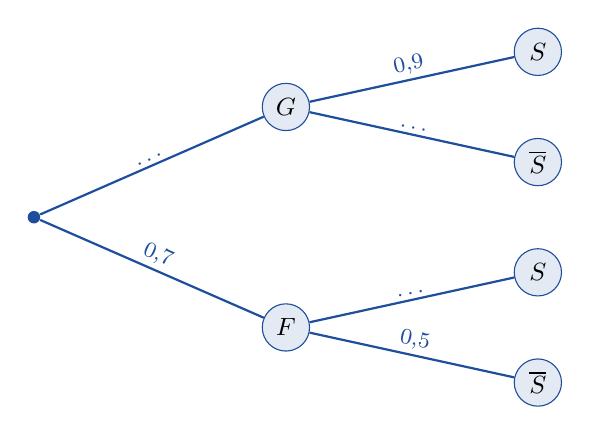
\begin{tikzpicture}[ev/.style={rounded rectangle,fill=cDef!12,draw=cDef,inner sep=2pt,minimum height=6mm,minimum width=7mm,font=\small},pb/.style={midway,above,sloped,font=\footnotesize,inner sep=1.5pt}]
\node[circle,fill=cDef,inner sep=1.6pt] (r) at (0,-2.10){};
\node[ev] (a0) at (3.20,-0.70){$G$};
\draw[cDef,thick] (r)--(a0) node[pb]{$\ldots$};
\node[ev] (b00) at (6.40,-0.00){$S$};
\draw[cDef,thick] (a0)--(b00) node[pb]{$0,9$};
\node[ev] (b01) at (6.40,-1.40){$\overline S$};
\draw[cDef,thick] (a0)--(b01) node[pb]{$\ldots$};
\node[ev] (a1) at (3.20,-3.50){$F$};
\draw[cDef,thick] (r)--(a1) node[pb]{$0,7$};
\node[ev] (b10) at (6.40,-2.80){$S$};
\draw[cDef,thick] (a1)--(b10) node[pb]{$\ldots$};
\node[ev] (b11) at (6.40,-4.20){$\overline S$};
\draw[cDef,thick] (a1)--(b11) node[pb]{$0,5$};
\end{tikzpicture}\end{LTR}\end{center}
\end{tamrin}
\begin{hal}
\QQ{1} $P(G)=1-0{,}7=0{,}3$ ، $P_G\big(\overline S\big)=1-0{,}9=0{,}1$ ، $P_F(S)=1-0{,}5=0{,}5$:
\par\begin{center}\begin{LTR}\begin{tikzpicture}[ev/.style={rounded rectangle,fill=cDef!12,draw=cDef,inner sep=2pt,minimum height=6mm,minimum width=7mm,font=\small},pb/.style={midway,above,sloped,font=\footnotesize,inner sep=1.5pt}]
\node[circle,fill=cDef,inner sep=1.6pt] (r) at (0,-2.10){};
\node[font=\small\bfseries,text=cSec] at (8.70,0.90){\ar{الاحتمال}};
\node[ev] (a0) at (3.20,-0.70){$G$};
\draw[cDef,thick] (r)--(a0) node[pb]{$0,3$};
\node[ev] (b00) at (6.40,-0.00){$S$};
\draw[cDef,thick] (a0)--(b00) node[pb]{$0,9$};
\node[font=\small] at (8.70,-0.00){$0,27$};
\node[ev] (b01) at (6.40,-1.40){$\overline S$};
\draw[cDef,thick] (a0)--(b01) node[pb]{$0,1$};
\node[font=\small] at (8.70,-1.40){$0,03$};
\node[ev] (a1) at (3.20,-3.50){$F$};
\draw[cDef,thick] (r)--(a1) node[pb]{$0,7$};
\node[ev] (b10) at (6.40,-2.80){$S$};
\draw[cDef,thick] (a1)--(b10) node[pb]{$0,5$};
\node[font=\small] at (8.70,-2.80){$0,35$};
\node[ev] (b11) at (6.40,-4.20){$\overline S$};
\draw[cDef,thick] (a1)--(b11) node[pb]{$0,5$};
\node[font=\small] at (8.70,-4.20){$0,35$};
\end{tikzpicture}\end{LTR}\end{center}
\QQ{2} $P(S)=0{,}27+0{,}35=\bx{0{,}62}$ \ ؛ \ $P\big(G\cap\overline S\big)=0{,}3\times0{,}1=\bx{0{,}03}$ ؛ \ $P\big(\overline S\big)=1-0{,}62=0{,}38$:
\[P_{\overline S}(F)=\frac{P\big(F\cap\overline S\big)}{P\big(\overline S\big)}=\frac{0{,}35}{0{,}38}=\bx{\frac{35}{38}}\qquad;\qquad P_S(G)=\frac{0{,}27}{0{,}62}=\bx{\frac{27}{62}}\]
\QQ{3} $P(G)\times P\big(\overline S\big)=0{,}3\times0{,}38=0{,}114\neq0{,}03=P\big(G\cap\overline S\big)$: \bxt{$G$ و $\overline S$ غير مستقلتين}.
\end{hal}
% ===================== 4 =====================
\begin{tamrin}{تمرين من بكالوريا 2018 -- الموضوع الثاني}
تضم مؤسسة إنتاجية موظفين من الجنسين: رجالًا يرمز لهم بـ $H$ ونساء يرمز لهن بـ $F$ ، منهم الإداريون $A$ والمهندسون $I$ والعمال $T$ ، موزعين حسب الجدول التالي:
\begin{center}\begin{LTR}\renewcommand{\arraystretch}{1.4}
\begin{tabular}{|C|c|c|c|}\hline
\rowcolor{cSec!12} & \ar{الإداريون} $A$ & \ar{المهندسون} $I$ & \ar{العمال} $T$\\\hline
الرجال & $12\%$ & $13\%$ & $27\%$\\\hline
النساء & $16\%$ & $12\%$ & $20\%$\\\hline
\end{tabular}\end{LTR}\end{center}
يخضع الموظفون لفحص طبي دوري. نختار عشوائيًا موظفًا.
\QQ{1}
\begin{sq}
\qa بيّن أن احتمال أن يكون الموظف رجلًا هو $P(H)=0{,}52$.
\qb أنقل ثم أتمم شجرة الاحتمالات.
\end{sq}
\QQ{2} احسب $P(H\cap T)$ و $P(F\cap I)$.
\QQ{3} ما احتمال أن يكون الموظف مهندسًا؟
\QQ{4} ما احتمال أن يكون الموظف رجلًا علمًا أنه إداري؟
\par\begin{center}\begin{LTR}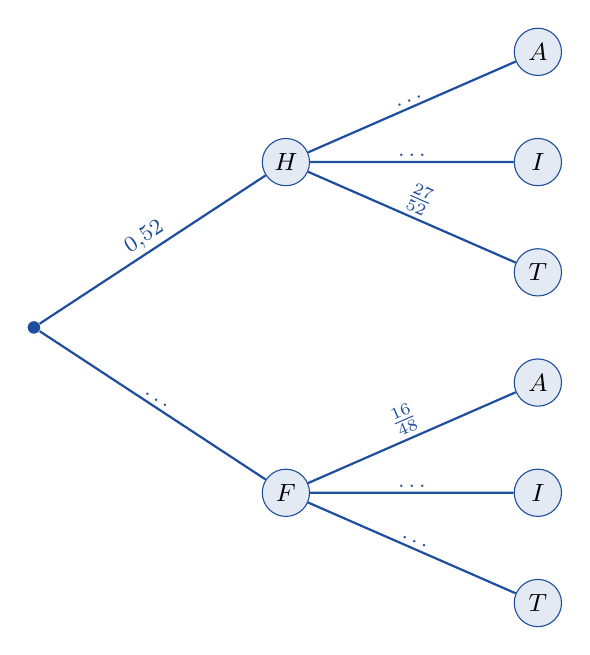
\begin{tikzpicture}[ev/.style={rounded rectangle,fill=cDef!12,draw=cDef,inner sep=2pt,minimum height=6mm,minimum width=7mm,font=\small},pb/.style={midway,above,sloped,font=\footnotesize,inner sep=1.5pt}]
\node[circle,fill=cDef,inner sep=1.6pt] (r) at (0,-3.50){};
\node[ev] (a0) at (3.20,-1.40){$H$};
\draw[cDef,thick] (r)--(a0) node[pb]{$0,52$};
\node[ev] (b00) at (6.40,-0.00){$A$};
\draw[cDef,thick] (a0)--(b00) node[pb]{$\ldots$};
\node[ev] (b01) at (6.40,-1.40){$I$};
\draw[cDef,thick] (a0)--(b01) node[pb]{$\ldots$};
\node[ev] (b02) at (6.40,-2.80){$T$};
\draw[cDef,thick] (a0)--(b02) node[pb]{$\frac{27}{52}$};
\node[ev] (a1) at (3.20,-5.60){$F$};
\draw[cDef,thick] (r)--(a1) node[pb]{$\ldots$};
\node[ev] (b10) at (6.40,-4.20){$A$};
\draw[cDef,thick] (a1)--(b10) node[pb]{$\frac{16}{48}$};
\node[ev] (b11) at (6.40,-5.60){$I$};
\draw[cDef,thick] (a1)--(b11) node[pb]{$\ldots$};
\node[ev] (b12) at (6.40,-7.00){$T$};
\draw[cDef,thick] (a1)--(b12) node[pb]{$\ldots$};
\end{tikzpicture}\end{LTR}\end{center}
\end{tamrin}
\begin{hal}
\QQ{1}
\pa $P(H)=0{,}12+0{,}13+0{,}27=\bx{0{,}52}$ ، و $P(F)=0{,}48$.
\pb $P_H(A)=\dfrac{0{,}12}{0{,}52}=\dfrac{12}{52}$ ، $\ldots$
\par\begin{center}\begin{LTR}\begin{tikzpicture}[ev/.style={rounded rectangle,fill=cDef!12,draw=cDef,inner sep=2pt,minimum height=6mm,minimum width=7mm,font=\small},pb/.style={midway,above,sloped,font=\footnotesize,inner sep=1.5pt}]
\node[circle,fill=cDef,inner sep=1.6pt] (r) at (0,-3.50){};
\node[font=\small\bfseries,text=cSec] at (8.70,0.90){\ar{الاحتمال}};
\node[ev] (a0) at (3.20,-1.40){$H$};
\draw[cDef,thick] (r)--(a0) node[pb]{$0,52$};
\node[ev] (b00) at (6.40,-0.00){$A$};
\draw[cDef,thick] (a0)--(b00) node[pb]{$\frac{12}{52}$};
\node[font=\small] at (8.70,-0.00){$0,12$};
\node[ev] (b01) at (6.40,-1.40){$I$};
\draw[cDef,thick] (a0)--(b01) node[pb]{$\frac{13}{52}$};
\node[font=\small] at (8.70,-1.40){$0,13$};
\node[ev] (b02) at (6.40,-2.80){$T$};
\draw[cDef,thick] (a0)--(b02) node[pb]{$\frac{27}{52}$};
\node[font=\small] at (8.70,-2.80){$0,27$};
\node[ev] (a1) at (3.20,-5.60){$F$};
\draw[cDef,thick] (r)--(a1) node[pb]{$0,48$};
\node[ev] (b10) at (6.40,-4.20){$A$};
\draw[cDef,thick] (a1)--(b10) node[pb]{$\frac{16}{48}$};
\node[font=\small] at (8.70,-4.20){$0,16$};
\node[ev] (b11) at (6.40,-5.60){$I$};
\draw[cDef,thick] (a1)--(b11) node[pb]{$\frac{12}{48}$};
\node[font=\small] at (8.70,-5.60){$0,12$};
\node[ev] (b12) at (6.40,-7.00){$T$};
\draw[cDef,thick] (a1)--(b12) node[pb]{$\frac{20}{48}$};
\node[font=\small] at (8.70,-7.00){$0,20$};
\end{tikzpicture}\end{LTR}\end{center}
\QQ{2} $P(H\cap T)=\bx{0{,}27}$ \ ؛ \ $P(F\cap I)=\bx{0{,}12}$
\QQ{3} $P(I)=0{,}13+0{,}12=\bx{0{,}25}$
\QQ{4} $P(A)=0{,}12+0{,}16=0{,}28$: \quad $P_A(H)=\dfrac{0{,}12}{0{,}28}=\bx{\frac37}$
\end{hal}
% ===================== 5 =====================
\begin{tamrin}{تمرين من بكالوريا 2017 -- الدورة الاستثنائية -- الموضوع الأول}
الشجرة التالية تنمذج تجربة عشوائية حيث $A$ و $B$ حادثتان ، $\overline A$ و $\overline B$ حادثتاهما العكسيتان على الترتيب ، و: $P(A)=0{,}35$ ، $P_A(B)=0{,}45$ ، $P_{\overline A}(B)=0{,}55$.
\QQ{1} أنقل وأكمل الشجرة ، ثم احسب الاحتمالين: $P\big(A\cap\overline B\big)$ و $P(A\cap B)$.
\par\begin{center}\begin{LTR}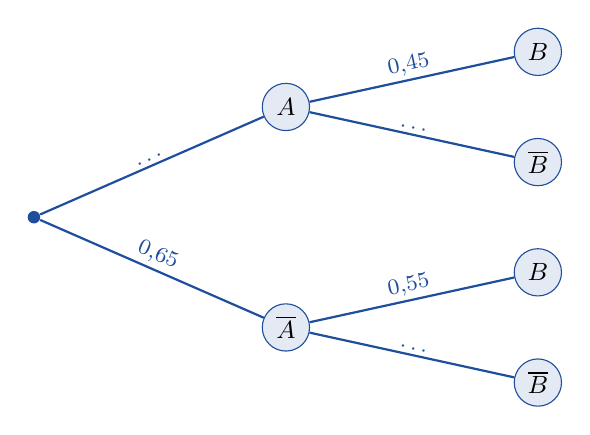
\begin{tikzpicture}[ev/.style={rounded rectangle,fill=cDef!12,draw=cDef,inner sep=2pt,minimum height=6mm,minimum width=7mm,font=\small},pb/.style={midway,above,sloped,font=\footnotesize,inner sep=1.5pt}]
\node[circle,fill=cDef,inner sep=1.6pt] (r) at (0,-2.10){};
\node[ev] (a0) at (3.20,-0.70){$A$};
\draw[cDef,thick] (r)--(a0) node[pb]{$\ldots$};
\node[ev] (b00) at (6.40,-0.00){$B$};
\draw[cDef,thick] (a0)--(b00) node[pb]{$0,45$};
\node[ev] (b01) at (6.40,-1.40){$\overline B$};
\draw[cDef,thick] (a0)--(b01) node[pb]{$\ldots$};
\node[ev] (a1) at (3.20,-3.50){$\overline A$};
\draw[cDef,thick] (r)--(a1) node[pb]{$0,65$};
\node[ev] (b10) at (6.40,-2.80){$B$};
\draw[cDef,thick] (a1)--(b10) node[pb]{$0,55$};
\node[ev] (b11) at (6.40,-4.20){$\overline B$};
\draw[cDef,thick] (a1)--(b11) node[pb]{$\ldots$};
\end{tikzpicture}\end{LTR}\end{center}
\QQ{2}
\begin{sq}
\qa احسب الاحتمالات الآتية: $P(B)$ ، $P_B(A)$ و $P_{\overline B}(A)$.
\qb أنقل وأكمل الشجرة التي تبدأ بالحادثتين $B$ و $\overline B$.
\end{sq}
\par\begin{center}\begin{LTR}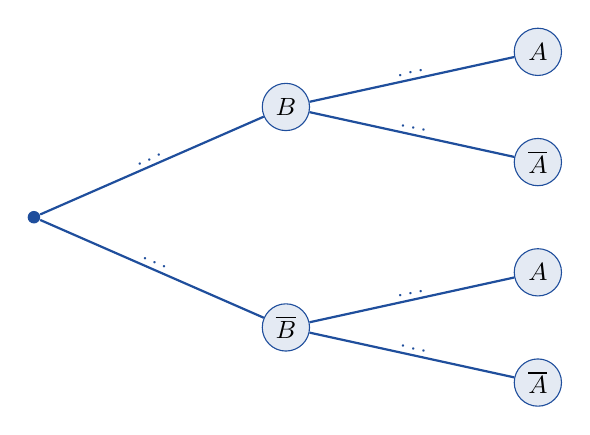
\begin{tikzpicture}[ev/.style={rounded rectangle,fill=cDef!12,draw=cDef,inner sep=2pt,minimum height=6mm,minimum width=7mm,font=\small},pb/.style={midway,above,sloped,font=\footnotesize,inner sep=1.5pt}]
\node[circle,fill=cDef,inner sep=1.6pt] (r) at (0,-2.10){};
\node[ev] (a0) at (3.20,-0.70){$B$};
\draw[cDef,thick] (r)--(a0) node[pb]{$\ldots$};
\node[ev] (b00) at (6.40,-0.00){$A$};
\draw[cDef,thick] (a0)--(b00) node[pb]{$\ldots$};
\node[ev] (b01) at (6.40,-1.40){$\overline A$};
\draw[cDef,thick] (a0)--(b01) node[pb]{$\ldots$};
\node[ev] (a1) at (3.20,-3.50){$\overline B$};
\draw[cDef,thick] (r)--(a1) node[pb]{$\ldots$};
\node[ev] (b10) at (6.40,-2.80){$A$};
\draw[cDef,thick] (a1)--(b10) node[pb]{$\ldots$};
\node[ev] (b11) at (6.40,-4.20){$\overline A$};
\draw[cDef,thick] (a1)--(b11) node[pb]{$\ldots$};
\end{tikzpicture}\end{LTR}\end{center}
\end{tamrin}
\begin{hal}
\QQ{1} $P\big(\overline A\big)=0{,}65$:
\par\begin{center}\begin{LTR}\begin{tikzpicture}[ev/.style={rounded rectangle,fill=cDef!12,draw=cDef,inner sep=2pt,minimum height=6mm,minimum width=7mm,font=\small},pb/.style={midway,above,sloped,font=\footnotesize,inner sep=1.5pt}]
\node[circle,fill=cDef,inner sep=1.6pt] (r) at (0,-2.10){};
\node[font=\small\bfseries,text=cSec] at (8.70,0.90){\ar{الاحتمال}};
\node[ev] (a0) at (3.20,-0.70){$A$};
\draw[cDef,thick] (r)--(a0) node[pb]{$0,35$};
\node[ev] (b00) at (6.40,-0.00){$B$};
\draw[cDef,thick] (a0)--(b00) node[pb]{$0,45$};
\node[font=\small] at (8.70,-0.00){$0,1575$};
\node[ev] (b01) at (6.40,-1.40){$\overline B$};
\draw[cDef,thick] (a0)--(b01) node[pb]{$0,55$};
\node[font=\small] at (8.70,-1.40){$0,1925$};
\node[ev] (a1) at (3.20,-3.50){$\overline A$};
\draw[cDef,thick] (r)--(a1) node[pb]{$0,65$};
\node[ev] (b10) at (6.40,-2.80){$B$};
\draw[cDef,thick] (a1)--(b10) node[pb]{$0,55$};
\node[font=\small] at (8.70,-2.80){$0,3575$};
\node[ev] (b11) at (6.40,-4.20){$\overline B$};
\draw[cDef,thick] (a1)--(b11) node[pb]{$0,45$};
\node[font=\small] at (8.70,-4.20){$0,2925$};
\end{tikzpicture}\end{LTR}\end{center}
$P(A\cap B)=0{,}35\times0{,}45=\bx{0{,}1575}$ \ ؛ \ $P\big(A\cap\overline B\big)=0{,}35\times0{,}55=\bx{0{,}1925}$
\QQ{2}
\pa $P(B)=0{,}1575+0{,}3575=\bx{0{,}515}$ \ ، \ $P\big(\overline B\big)=0{,}485$:
\[P_B(A)=\frac{0{,}1575}{0{,}515}=\bx{\frac{63}{206}}\qquad;\qquad P_{\overline B}(A)=\frac{0{,}1925}{0{,}485}=\bx{\frac{77}{194}}\]
\pb
\par\begin{center}\begin{LTR}\begin{tikzpicture}[ev/.style={rounded rectangle,fill=cDef!12,draw=cDef,inner sep=2pt,minimum height=6mm,minimum width=7mm,font=\small},pb/.style={midway,above,sloped,font=\footnotesize,inner sep=1.5pt}]
\node[circle,fill=cDef,inner sep=1.6pt] (r) at (0,-2.10){};
\node[font=\small\bfseries,text=cSec] at (8.70,0.90){\ar{الاحتمال}};
\node[ev] (a0) at (3.20,-0.70){$B$};
\draw[cDef,thick] (r)--(a0) node[pb]{$0,515$};
\node[ev] (b00) at (6.40,-0.00){$A$};
\draw[cDef,thick] (a0)--(b00) node[pb]{$\frac{63}{206}$};
\node[font=\small] at (8.70,-0.00){$0,1575$};
\node[ev] (b01) at (6.40,-1.40){$\overline A$};
\draw[cDef,thick] (a0)--(b01) node[pb]{$\frac{143}{206}$};
\node[font=\small] at (8.70,-1.40){$0,3575$};
\node[ev] (a1) at (3.20,-3.50){$\overline B$};
\draw[cDef,thick] (r)--(a1) node[pb]{$0,485$};
\node[ev] (b10) at (6.40,-2.80){$A$};
\draw[cDef,thick] (a1)--(b10) node[pb]{$\frac{77}{194}$};
\node[font=\small] at (8.70,-2.80){$0,1925$};
\node[ev] (b11) at (6.40,-4.20){$\overline A$};
\draw[cDef,thick] (a1)--(b11) node[pb]{$\frac{117}{194}$};
\node[font=\small] at (8.70,-4.20){$0,2925$};
\end{tikzpicture}\end{LTR}\end{center}
\end{hal}
% ===================== 6 =====================
\begin{tamrin}{تمرين من بكالوريا 2017 -- الدورة الاستثنائية -- الموضوع الثاني}
في كل حالة من الحالات الآتية ، اقترحت ثلاث إجابات واحدة منها فقط صحيحة ، عيّن الاقتراح الصحيح مع التبرير:
\QQ{1} $A$ و $B$ حادثتان مستقلتان. إذا كان $P(A)=0{,}4$ و $P(A\cap B)=0{,}03$ فإن: \ABC{$P(B)=0{,}43$}{$P(B)=0{,}075$}{$P(B)=0{,}37$}
\QQ{2} $A$ و $B$ حادثتان. إذا كان $P(A\cap B)=\dfrac3{100}$ و $P_A(B)=\dfrac14$ فإن: \ABC{$P(A)=\dfrac3{25}$}{$P(A)=\dfrac4{25}$}{$P(A)=\dfrac3{400}$}
\QQ{3} $A$ و $B$ حادثتان. إذا كان $P(A)=0{,}4$ ، $P(B)=0{,}5$ و $P\big(\overline{A\cup B}\big)=0{,}55$ فإن: \ABC{$P(A\cap B)=0{,}2$}{$P(A\cap B)=0{,}45$}{$P(A\cap B)=0{,}9$}
\QQ{4} الجدول التالي يعرّف قانون احتمال تجربة عشوائية:
\begin{center}\begin{LTR}\renewcommand{\arraystretch}{1.4}
\begin{tabular}{|c|c|c|c|c|}\hline
\rowcolor{cSec!12}$x_i$ & $-2$ & $-1$ & $\alpha$ & $3$\\\hline
$P(X=x_i)$ & $0{,}12$ & $0{,}50$ & $\beta$ & $0{,}30$\\\hline
\end{tabular}\end{LTR}\end{center}
قيمتا $\alpha$ و $\beta$ حتى يكون الأمل الرياضياتي للمتغير العشوائي $X$ يساوي $0{,}32$ هما: \ABC{$\alpha=1$ و $\beta=0{,}08$}{$\alpha=2$ و $\beta=0{,}03$}{$\alpha=2$ و $\beta=0{,}08$}
\end{tamrin}
\begin{hal}
\QQ{1} $P(A\cap B)=P(A)\times P(B)$ ، ومنه $P(B)=\dfrac{0{,}03}{0{,}4}=0{,}075$: \bxt{الجواب (ب)}.
\QQ{2} $P(A\cap B)=P(A)\times P_A(B)$ ، ومنه $P(A)=\dfrac{3}{100}\times4=\dfrac{12}{100}=\dfrac3{25}$: \bxt{الجواب (أ)}.
\QQ{3} $P(A\cup B)=1-0{,}55=0{,}45$ ، و $P(A\cap B)=P(A)+P(B)-P(A\cup B)=0{,}4+0{,}5-0{,}45=0{,}45$: \bxt{الجواب (ب)}.
\QQ{4} $0{,}12+0{,}50+\beta+0{,}30=1$ ، ومنه $\beta=0{,}08$. \ $E(X)=-0{,}24-0{,}5+0{,}08\alpha+0{,}9=0{,}16+0{,}08\alpha=0{,}32$ ، ومنه $\alpha=2$: \bxt{الجواب (جـ)}.
\end{hal}
% ===================== 7 =====================
\begin{tamrin}{تمرين من بكالوريا 2017 -- الموضوع الأول}
يستقبل مركز إجراء امتحان شهادة البكالوريا مترشحين موزعين على ثلاث شعب هي: شعبة الآداب والفلسفة $(L)$ ، شعبة العلوم التجريبية $(S)$ ، شعبة التسيير والاقتصاد $(G)$. \ $47\%$ من المترشحين ذكور $(M)$ والباقي إناث $(F)$.
\par من بين الذكور يوجد $35\%$ في شعبة العلوم التجريبية و $49\%$ في شعبة الآداب والفلسفة. ومن بين الإناث يوجد $10\%$ في شعبة التسيير والاقتصاد و $37\%$ في العلوم التجريبية. نختار عشوائيًا مترشحًا من هذا المركز.
\QQ{1} أنجز شجرة الاحتمالات التي تنمذج هذه الوضعية.
\QQ{2} احسب احتمال كل حادثة مما يلي:
\par $A$: «المترشح المختار أنثى ومن شعبة التسيير والاقتصاد» ؛ \ $B$: «المترشح المختار من شعبة التسيير والاقتصاد» ؛ \ $C$: «المترشح المختار أنثى علمًا أنه من شعبة التسيير والاقتصاد».
\end{tamrin}
\begin{hal}
\QQ{1} $P(F)=0{,}53$ ، $P_M(G)=1-0{,}35-0{,}49=0{,}16$ ، $P_F(L)=1-0{,}10-0{,}37=0{,}53$:
\par\begin{center}\begin{LTR}\begin{tikzpicture}[ev/.style={rounded rectangle,fill=cDef!12,draw=cDef,inner sep=2pt,minimum height=6mm,minimum width=7mm,font=\small},pb/.style={midway,above,sloped,font=\footnotesize,inner sep=1.5pt}]
\node[circle,fill=cDef,inner sep=1.6pt] (r) at (0,-3.50){};
\node[font=\small\bfseries,text=cSec] at (8.70,0.90){\ar{الاحتمال}};
\node[ev] (a0) at (3.20,-1.40){$M$};
\draw[cDef,thick] (r)--(a0) node[pb]{$0,47$};
\node[ev] (b00) at (6.40,-0.00){$S$};
\draw[cDef,thick] (a0)--(b00) node[pb]{$0,35$};
\node[font=\small] at (8.70,-0.00){$0,1645$};
\node[ev] (b01) at (6.40,-1.40){$L$};
\draw[cDef,thick] (a0)--(b01) node[pb]{$0,49$};
\node[font=\small] at (8.70,-1.40){$0,2303$};
\node[ev] (b02) at (6.40,-2.80){$G$};
\draw[cDef,thick] (a0)--(b02) node[pb]{$0,16$};
\node[font=\small] at (8.70,-2.80){$0,0752$};
\node[ev] (a1) at (3.20,-5.60){$F$};
\draw[cDef,thick] (r)--(a1) node[pb]{$0,53$};
\node[ev] (b10) at (6.40,-4.20){$S$};
\draw[cDef,thick] (a1)--(b10) node[pb]{$0,37$};
\node[font=\small] at (8.70,-4.20){$0,1961$};
\node[ev] (b11) at (6.40,-5.60){$L$};
\draw[cDef,thick] (a1)--(b11) node[pb]{$0,53$};
\node[font=\small] at (8.70,-5.60){$0,2809$};
\node[ev] (b12) at (6.40,-7.00){$G$};
\draw[cDef,thick] (a1)--(b12) node[pb]{$0,10$};
\node[font=\small] at (8.70,-7.00){$0,053$};
\end{tikzpicture}\end{LTR}\end{center}
\QQ{2} $P(A)=P(F\cap G)=0{,}53\times0{,}10=\bx{0{,}053}$ \ ؛ \ $P(B)=P(G)=0{,}0752+0{,}053=\bx{0{,}1282}$
\[P(C)=P_G(F)=\frac{0{,}053}{0{,}1282}=\bx{\frac{265}{641}}\approx0{,}41\]
\end{hal}
% ===================== 8 =====================
\begin{tamrin}{تمرين من بكالوريا 2017 -- الموضوع الثاني}
أجريت دراسة حول العلاقة بين استعمال الأنترنت وامتلاك جهاز حاسوب في مدينة ما ، فكانت النتائج كما يلي: $80\%$ من سكان هذه المدينة يملكون جهاز حاسوب ، $90\%$ من سكان هذه المدينة الذين يملكون جهاز حاسوب يستعملون الأنترنت ، $60\%$ من سكان هذه المدينة الذين لا يملكون جهاز حاسوب لا يستعملون الأنترنت.
\par نختار عشوائيًا شخصًا من هذه المدينة. نرمز بـ $A$ إلى الحادثة «الشخص المختار يملك جهاز حاسوب» ، وبـ $B$ إلى الحادثة «الشخص المختار يستعمل الأنترنت».
\QQ{1} أنجز شجرة الاحتمالات التي تنمذج هذه الوضعية.
\QQ{2}
\begin{sq}
\qa بيّن أن احتمال أن يكون الشخص المختار لا يملك جهاز حاسوب يساوي $0{,}20$.
\qb ما احتمال أن يكون الشخص المختار يملك جهاز حاسوب ويستعمل الأنترنت؟
\qc ما احتمال أن يكون الشخص المختار لا يملك جهاز حاسوب ويستعمل الأنترنت؟
\end{sq}
\QQ{3} احسب احتمال أن يكون الشخص المختار يستعمل الأنترنت.
\QQ{4} احسب احتمال أن يكون الشخص المختار يملك جهاز حاسوب علمًا أنه يستعمل الأنترنت.
\end{tamrin}
\begin{hal}
\QQ{1}
\par\begin{center}\begin{LTR}\begin{tikzpicture}[ev/.style={rounded rectangle,fill=cDef!12,draw=cDef,inner sep=2pt,minimum height=6mm,minimum width=7mm,font=\small},pb/.style={midway,above,sloped,font=\footnotesize,inner sep=1.5pt}]
\node[circle,fill=cDef,inner sep=1.6pt] (r) at (0,-2.10){};
\node[font=\small\bfseries,text=cSec] at (8.70,0.90){\ar{الاحتمال}};
\node[ev] (a0) at (3.20,-0.70){$A$};
\draw[cDef,thick] (r)--(a0) node[pb]{$0,8$};
\node[ev] (b00) at (6.40,-0.00){$B$};
\draw[cDef,thick] (a0)--(b00) node[pb]{$0,9$};
\node[font=\small] at (8.70,-0.00){$0,72$};
\node[ev] (b01) at (6.40,-1.40){$\overline B$};
\draw[cDef,thick] (a0)--(b01) node[pb]{$0,1$};
\node[font=\small] at (8.70,-1.40){$0,08$};
\node[ev] (a1) at (3.20,-3.50){$\overline A$};
\draw[cDef,thick] (r)--(a1) node[pb]{$0,2$};
\node[ev] (b10) at (6.40,-2.80){$B$};
\draw[cDef,thick] (a1)--(b10) node[pb]{$0,4$};
\node[font=\small] at (8.70,-2.80){$0,08$};
\node[ev] (b11) at (6.40,-4.20){$\overline B$};
\draw[cDef,thick] (a1)--(b11) node[pb]{$0,6$};
\node[font=\small] at (8.70,-4.20){$0,12$};
\end{tikzpicture}\end{LTR}\end{center}
\QQ{2}
\pa $P\big(\overline A\big)=1-0{,}8=\bx{0{,}20}$
\pb $P(A\cap B)=0{,}8\times0{,}9=\bx{0{,}72}$
\pc $P\big(\overline A\cap B\big)=0{,}2\times0{,}4=\bx{0{,}08}$
\QQ{3} $P(B)=0{,}72+0{,}08=\bx{0{,}8}$
\QQ{4} $P_B(A)=\dfrac{0{,}72}{0{,}8}=\bx{0{,}9}$
\end{hal}
% ===================== 9 =====================
\begin{tamrin}{تمرين من بكالوريا 2016 -- الموضوع الأول}
الجدول التالي يعطي توزيع $500$ تلميذ في إحدى الثانويات:
\begin{center}\begin{LTR}\renewcommand{\arraystretch}{1.4}
\begin{tabular}{|C|c|c|c|}\hline
\rowcolor{cSec!12}التلميذ & \ar{ذكور} & \ar{إناث} & \ar{المجموع}\\\hline
يملك هاتفًا نقالًا & $60$ & $240$ & $300$\\\hline
لا يملك هاتفًا نقالًا & $120$ & $80$ & $200$\\\hline
المجموع & $180$ & $320$ & $500$\\\hline
\end{tabular}\end{LTR}\end{center}
نختار عشوائيًا تلميذًا من الثانوية ونسمي الحادثة $H$: «التلميذ المختار ذكر» ، الحادثة $F$: «التلميذ المختار أنثى» ، الحادثة $S$: «التلميذ يملك هاتفًا نقالًا» ، الحادثة $\overline S$: «التلميذ لا يملك هاتفًا نقالًا».
\QQ{1} شكّل شجرة الاحتمالات لهذه التجربة.
\QQ{2} احسب احتمال الحوادث التالية:
\begin{sq}
\qa التلميذ المختار أنثى وتملك هاتفًا نقالًا.
\qb التلميذ المختار لا يملك هاتفًا نقالًا.
\end{sq}
\QQ{3} نفرض أن التلميذ المختار لا يملك هاتفًا نقالًا. ما هو احتمال أن يكون هذا التلميذ ذكرًا؟
\end{tamrin}
\begin{hal}
\QQ{1} $P(H)=\dfrac{180}{500}=\dfrac9{25}$ ، $P_H(S)=\dfrac{60}{180}=\dfrac13$ ، $P_F(S)=\dfrac{240}{320}=\dfrac34$:
\par\begin{center}\begin{LTR}\begin{tikzpicture}[ev/.style={rounded rectangle,fill=cDef!12,draw=cDef,inner sep=2pt,minimum height=6mm,minimum width=7mm,font=\small},pb/.style={midway,above,sloped,font=\footnotesize,inner sep=1.5pt}]
\node[circle,fill=cDef,inner sep=1.6pt] (r) at (0,-2.10){};
\node[font=\small\bfseries,text=cSec] at (8.70,0.90){\ar{الاحتمال}};
\node[ev] (a0) at (3.20,-0.70){$H$};
\draw[cDef,thick] (r)--(a0) node[pb]{$\frac{9}{25}$};
\node[ev] (b00) at (6.40,-0.00){$S$};
\draw[cDef,thick] (a0)--(b00) node[pb]{$\frac13$};
\node[font=\small] at (8.70,-0.00){$\frac{3}{25}$};
\node[ev] (b01) at (6.40,-1.40){$\overline S$};
\draw[cDef,thick] (a0)--(b01) node[pb]{$\frac23$};
\node[font=\small] at (8.70,-1.40){$\frac{6}{25}$};
\node[ev] (a1) at (3.20,-3.50){$F$};
\draw[cDef,thick] (r)--(a1) node[pb]{$\frac{16}{25}$};
\node[ev] (b10) at (6.40,-2.80){$S$};
\draw[cDef,thick] (a1)--(b10) node[pb]{$\frac34$};
\node[font=\small] at (8.70,-2.80){$\frac{12}{25}$};
\node[ev] (b11) at (6.40,-4.20){$\overline S$};
\draw[cDef,thick] (a1)--(b11) node[pb]{$\frac14$};
\node[font=\small] at (8.70,-4.20){$\frac{4}{25}$};
\end{tikzpicture}\end{LTR}\end{center}
\QQ{2}
\pa $P(F\cap S)=\dfrac{240}{500}=\bx{\frac{12}{25}}$
\pb $P\big(\overline S\big)=\dfrac{200}{500}=\bx{\frac25}$
\QQ{3} $P_{\overline S}(H)=\dfrac{120}{200}=\bx{\frac35}$
\end{hal}
% ===================== 10 =====================
\begin{tamrin}{تمرين من بكالوريا 2016 -- الموضوع الثاني}
وكالة أسفار تقترح على زبائنها ثلاث وجهات $A$ ، $B$ و $C$. \ $20\%$ من الزبائن اختاروا الوجهة $A$ ، $50\%$ اختاروا الوجهة $B$ والباقي اختار الوجهة $C$.
\par عند العودة من السفر أجرت الوكالة استجوابًا لزبائنها حول مدى إعجابهم بالوجهة ، واستنتجت ما يلي: $50\%$ من أصحاب الوجهة $A$ كانوا معجبين بها ، $30\%$ من أصحاب الوجهة $B$ كانوا غير معجبين بها ، $80\%$ من أصحاب الوجهة $C$ كانوا معجبين بها.
\par نختار عشوائيًا أحد الزبائن ونسجل الحوادث: $S$: «الزبون معجب بالوجهة المختارة» ، $\overline S$: «الزبون غير معجب بالوجهة المختارة».
\QQ{1} أنقل شجرة الاحتمالات ثم أكمل القيم الناقصة.
\QQ{2}
\begin{sq}
\qa احسب احتمالات الحوادث الآتية: $A\cap S$ ، $B\cap S$ ، $C\cap S$.
\qb استنتج احتمال أن يكون الزبون معجبًا بالوجهة المختارة.
\end{sq}
\QQ{3} نستجوب زبونًا غير معجب بالوجهة المختارة ، ما احتمال أن يكون من أصحاب الوجهة $B$ ؟
\par\begin{center}\begin{LTR}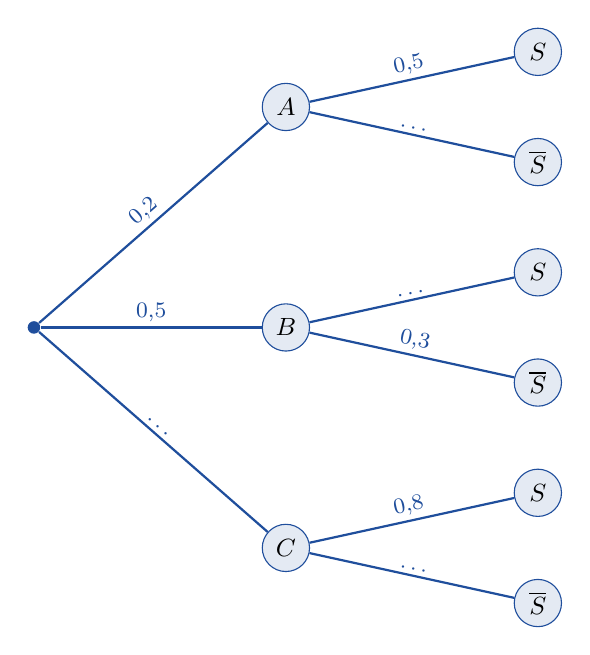
\begin{tikzpicture}[ev/.style={rounded rectangle,fill=cDef!12,draw=cDef,inner sep=2pt,minimum height=6mm,minimum width=7mm,font=\small},pb/.style={midway,above,sloped,font=\footnotesize,inner sep=1.5pt}]
\node[circle,fill=cDef,inner sep=1.6pt] (r) at (0,-3.50){};
\node[ev] (a0) at (3.20,-0.70){$A$};
\draw[cDef,thick] (r)--(a0) node[pb]{$0,2$};
\node[ev] (b00) at (6.40,-0.00){$S$};
\draw[cDef,thick] (a0)--(b00) node[pb]{$0,5$};
\node[ev] (b01) at (6.40,-1.40){$\overline S$};
\draw[cDef,thick] (a0)--(b01) node[pb]{$\ldots$};
\node[ev] (a1) at (3.20,-3.50){$B$};
\draw[cDef,thick] (r)--(a1) node[pb]{$0,5$};
\node[ev] (b10) at (6.40,-2.80){$S$};
\draw[cDef,thick] (a1)--(b10) node[pb]{$\ldots$};
\node[ev] (b11) at (6.40,-4.20){$\overline S$};
\draw[cDef,thick] (a1)--(b11) node[pb]{$0,3$};
\node[ev] (a2) at (3.20,-6.30){$C$};
\draw[cDef,thick] (r)--(a2) node[pb]{$\ldots$};
\node[ev] (b20) at (6.40,-5.60){$S$};
\draw[cDef,thick] (a2)--(b20) node[pb]{$0,8$};
\node[ev] (b21) at (6.40,-7.00){$\overline S$};
\draw[cDef,thick] (a2)--(b21) node[pb]{$\ldots$};
\end{tikzpicture}\end{LTR}\end{center}
\end{tamrin}
\begin{hal}
\QQ{1} $P(C)=1-0{,}2-0{,}5=0{,}3$ ، $P_A\big(\overline S\big)=0{,}5$ ، $P_B(S)=0{,}7$ ، $P_C\big(\overline S\big)=0{,}2$:
\par\begin{center}\begin{LTR}\begin{tikzpicture}[ev/.style={rounded rectangle,fill=cDef!12,draw=cDef,inner sep=2pt,minimum height=6mm,minimum width=7mm,font=\small},pb/.style={midway,above,sloped,font=\footnotesize,inner sep=1.5pt}]
\node[circle,fill=cDef,inner sep=1.6pt] (r) at (0,-3.50){};
\node[font=\small\bfseries,text=cSec] at (8.70,0.90){\ar{الاحتمال}};
\node[ev] (a0) at (3.20,-0.70){$A$};
\draw[cDef,thick] (r)--(a0) node[pb]{$0,2$};
\node[ev] (b00) at (6.40,-0.00){$S$};
\draw[cDef,thick] (a0)--(b00) node[pb]{$0,5$};
\node[font=\small] at (8.70,-0.00){$0,1$};
\node[ev] (b01) at (6.40,-1.40){$\overline S$};
\draw[cDef,thick] (a0)--(b01) node[pb]{$0,5$};
\node[font=\small] at (8.70,-1.40){$0,1$};
\node[ev] (a1) at (3.20,-3.50){$B$};
\draw[cDef,thick] (r)--(a1) node[pb]{$0,5$};
\node[ev] (b10) at (6.40,-2.80){$S$};
\draw[cDef,thick] (a1)--(b10) node[pb]{$0,7$};
\node[font=\small] at (8.70,-2.80){$0,35$};
\node[ev] (b11) at (6.40,-4.20){$\overline S$};
\draw[cDef,thick] (a1)--(b11) node[pb]{$0,3$};
\node[font=\small] at (8.70,-4.20){$0,15$};
\node[ev] (a2) at (3.20,-6.30){$C$};
\draw[cDef,thick] (r)--(a2) node[pb]{$0,3$};
\node[ev] (b20) at (6.40,-5.60){$S$};
\draw[cDef,thick] (a2)--(b20) node[pb]{$0,8$};
\node[font=\small] at (8.70,-5.60){$0,24$};
\node[ev] (b21) at (6.40,-7.00){$\overline S$};
\draw[cDef,thick] (a2)--(b21) node[pb]{$0,2$};
\node[font=\small] at (8.70,-7.00){$0,06$};
\end{tikzpicture}\end{LTR}\end{center}
\QQ{2}
\pa $P(A\cap S)=\bx{0{,}1}$ \ ؛ \ $P(B\cap S)=\bx{0{,}35}$ \ ؛ \ $P(C\cap S)=\bx{0{,}24}$
\pb $P(S)=0{,}1+0{,}35+0{,}24=\bx{0{,}69}$
\QQ{3} $P\big(\overline S\big)=0{,}31$ و $P\big(B\cap\overline S\big)=0{,}15$: \quad $P_{\overline S}(B)=\dfrac{0{,}15}{0{,}31}=\bx{\frac{15}{31}}$
\end{hal}
% ===================== 11 =====================
\begin{tamrin}{تمرين من بكالوريا 2015 -- الموضوع الثاني}
مصنع سيارات يشتغل بوحدتين $A$ و $B$ وينتج نوعين: سيارات تسير بالبنزين ويرمز إليها بـ $E$ وأخرى بغير البنزين $\overline E$. ربع إنتاج هذا المصنع تصنعه الوحدة $A$.
\par اشترى شخص سيارة من إنتاج هذا المصنع ، احتمال أن تكون هذه السيارة من صنع الوحدة $A$ وتسير بالبنزين يساوي $\dfrac16$ ، واحتمال أن تكون من صنع الوحدة $B$ وتسير بالبنزين يساوي $\dfrac38$. (تعطى كل النتائج على شكل كسر غير قابل للاختزال.)
\QQ{1} بيّن أن احتمال أن تكون السيارة تسير بالبنزين علمًا أنها من صنع الوحدة $A$ يساوي $\dfrac23$.
\QQ{2} احسب احتمال أن تكون السيارة تسير بالبنزين علمًا أنها من صنع الوحدة $B$.
\QQ{3}
\begin{sq}
\qa احسب احتمال أن تكون السيارة تسير بالبنزين.
\qb علمًا أن السيارة تسير بالبنزين ، ما احتمال أن تكون من صنع الوحدة $A$ ؟
\end{sq}
\QQ{4} أنجز شجرة الاحتمالات التي تنمذج هذه الوضعية.
\end{tamrin}
\begin{hal}
\QQ{1} $P(A)=\dfrac14$ ، $P(A\cap E)=\dfrac16$: \quad $P_A(E)=\dfrac{\frac16}{\frac14}=\bx{\frac23}$
\QQ{2} $P(B)=\dfrac34$: \quad $P_B(E)=\dfrac{\frac38}{\frac34}=\bx{\frac12}$
\QQ{3}
\pa $P(E)=\dfrac16+\dfrac38=\dfrac4{24}+\dfrac9{24}=\bx{\frac{13}{24}}$
\pb $P_E(A)=\dfrac{\frac16}{\frac{13}{24}}=\dfrac{24}{6\times13}=\bx{\frac4{13}}$
\QQ{4}
\par\begin{center}\begin{LTR}\begin{tikzpicture}[ev/.style={rounded rectangle,fill=cDef!12,draw=cDef,inner sep=2pt,minimum height=6mm,minimum width=7mm,font=\small},pb/.style={midway,above,sloped,font=\footnotesize,inner sep=1.5pt}]
\node[circle,fill=cDef,inner sep=1.6pt] (r) at (0,-2.10){};
\node[font=\small\bfseries,text=cSec] at (8.70,0.90){\ar{الاحتمال}};
\node[ev] (a0) at (3.20,-0.70){$A$};
\draw[cDef,thick] (r)--(a0) node[pb]{$\frac14$};
\node[ev] (b00) at (6.40,-0.00){$E$};
\draw[cDef,thick] (a0)--(b00) node[pb]{$\frac23$};
\node[font=\small] at (8.70,-0.00){$\frac16$};
\node[ev] (b01) at (6.40,-1.40){$\overline E$};
\draw[cDef,thick] (a0)--(b01) node[pb]{$\frac13$};
\node[font=\small] at (8.70,-1.40){$\frac1{12}$};
\node[ev] (a1) at (3.20,-3.50){$B$};
\draw[cDef,thick] (r)--(a1) node[pb]{$\frac34$};
\node[ev] (b10) at (6.40,-2.80){$E$};
\draw[cDef,thick] (a1)--(b10) node[pb]{$\frac12$};
\node[font=\small] at (8.70,-2.80){$\frac38$};
\node[ev] (b11) at (6.40,-4.20){$\overline E$};
\draw[cDef,thick] (a1)--(b11) node[pb]{$\frac12$};
\node[font=\small] at (8.70,-4.20){$\frac38$};
\end{tikzpicture}\end{LTR}\end{center}
\end{hal}
% ===================== 12 =====================
\begin{tamrin}{تمرين من بكالوريا 2014 -- الموضوع الأول}
ثلاثة أكياس متماثلة $U_1$ ، $U_2$ و $U_3$ كل منها يحوي $6$ كريات متماثلة: الكيس $U_1$ يحوي كريتين بيضاوين وأربع كريات حمراء ، الكيس $U_2$ يحوي ثلاث كريات بيضاء وثلاث كريات حمراء ، والكيس $U_3$ يحوي خمس كريات بيضاء وكرية حمراء. نختار عشوائيًا كيسًا ثم نسحب منه دون اختيار كرية واحدة.
\QQ{1} شكّل شجرة الاحتمالات المتوازنة التي تنمذج هذه الوضعية.
\QQ{2} ما احتمال سحب كرية بيضاء من الكيس $U_3$ ؟
\QQ{3} ما احتمال سحب كرية بيضاء؟
\QQ{4} علمًا أن الكرية المسحوبة بيضاء ، ما احتمال أن تكون من الكيس $U_3$ ؟
\end{tamrin}
\begin{hal}
\QQ{1} نرمز بـ $W$ للبيضاء و $R$ للحمراء:
\par\begin{center}\begin{LTR}\begin{tikzpicture}[ev/.style={rounded rectangle,fill=cDef!12,draw=cDef,inner sep=2pt,minimum height=6mm,minimum width=7mm,font=\small},pb/.style={midway,above,sloped,font=\footnotesize,inner sep=1.5pt}]
\node[circle,fill=cDef,inner sep=1.6pt] (r) at (0,-3.50){};
\node[font=\small\bfseries,text=cSec] at (8.70,0.90){\ar{الاحتمال}};
\node[ev] (a0) at (3.20,-0.70){$U_1$};
\draw[cDef,thick] (r)--(a0) node[pb]{$\frac13$};
\node[ev] (b00) at (6.40,-0.00){$W$};
\draw[cDef,thick] (a0)--(b00) node[pb]{$\frac26$};
\node[font=\small] at (8.70,-0.00){$\frac2{18}$};
\node[ev] (b01) at (6.40,-1.40){$R$};
\draw[cDef,thick] (a0)--(b01) node[pb]{$\frac46$};
\node[font=\small] at (8.70,-1.40){$\frac4{18}$};
\node[ev] (a1) at (3.20,-3.50){$U_2$};
\draw[cDef,thick] (r)--(a1) node[pb]{$\frac13$};
\node[ev] (b10) at (6.40,-2.80){$W$};
\draw[cDef,thick] (a1)--(b10) node[pb]{$\frac36$};
\node[font=\small] at (8.70,-2.80){$\frac3{18}$};
\node[ev] (b11) at (6.40,-4.20){$R$};
\draw[cDef,thick] (a1)--(b11) node[pb]{$\frac36$};
\node[font=\small] at (8.70,-4.20){$\frac3{18}$};
\node[ev] (a2) at (3.20,-6.30){$U_3$};
\draw[cDef,thick] (r)--(a2) node[pb]{$\frac13$};
\node[ev] (b20) at (6.40,-5.60){$W$};
\draw[cDef,thick] (a2)--(b20) node[pb]{$\frac56$};
\node[font=\small] at (8.70,-5.60){$\frac5{18}$};
\node[ev] (b21) at (6.40,-7.00){$R$};
\draw[cDef,thick] (a2)--(b21) node[pb]{$\frac16$};
\node[font=\small] at (8.70,-7.00){$\frac1{18}$};
\end{tikzpicture}\end{LTR}\end{center}
\QQ{2} $P(U_3\cap W)=\dfrac13\times\dfrac56=\bx{\frac5{18}}$
\QQ{3} $P(W)=\dfrac2{18}+\dfrac3{18}+\dfrac5{18}=\dfrac{10}{18}=\bx{\frac59}$
\QQ{4} $P_W(U_3)=\dfrac{\frac5{18}}{\frac{10}{18}}=\bx{\frac12}$
\end{hal}
% ===================== 13 =====================
\begin{tamrin}{تمرين من بكالوريا 2014 -- الموضوع الثاني}
عيّن مع التبرير الجواب الصحيح الوحيد من بين الأجوبة الثلاثة المقترحة في كل حالة من الحالات الآتية:
\par\textbf{I)} أعضاء الطاقم الصحي لمؤسسة استشفائية موزعين حسب الجدول التالي ، نختار عشوائيًا عضوًا من هذا الطاقم:
\begin{center}\begin{LTR}\renewcommand{\arraystretch}{1.4}
\begin{tabular}{|C|c|c|}\hline
\rowcolor{cSec!12} & \ar{أطباء} & \ar{ممرضون}\\\hline
ذكور & $12$ & $25$\\\hline
إناث & $8$ & $15$\\\hline
\end{tabular}\end{LTR}\end{center}
\QQ{1} احتمال أن يكون العضو المختار أنثى هو: \ABC{$\dfrac1{23}$}{$\dfrac{23}{60}$}{$\dfrac8{23}$}
\QQ{2} احتمال أن يكون العضو المختار أنثى علمًا أنها طبيبة هو: \ABC{$\dfrac25$}{$\dfrac2{15}$}{$\dfrac8{23}$}
\par\textbf{II)} الجدول التالي يعرّف قانون احتمال لتجربة عشوائية:
\begin{center}\begin{LTR}\renewcommand{\arraystretch}{1.4}
\begin{tabular}{|c|c|c|c|c|}\hline
\rowcolor{cSec!12}$x_i$ & $1$ & $2$ & $3$ & $4$\\\hline
$p_i$ & $0{,}2$ & $0{,}4$ & $0{,}1$ & $0{,}3$\\\hline
\end{tabular}\end{LTR}\end{center}
\QQ{1} تباين قانون الاحتمال هو: \ABC{$1{,}12$}{$2{,}5$}{$1{,}25$}
\QQ{2} إذا كانت $A$ و $B$ حادثتين مستقلتين حيث $P(A)=0{,}4$ ، $P(B)=0{,}3$ فإن $P(A\cap B)$ هو: \ABC{$0{,}12$}{$0{,}7$}{$0{,}75$}
\end{tamrin}
\begin{hal}
\textbf{I)} العدد الكلي: $12+25+8+15=60$.
\QQ{1} عدد الإناث $8+15=23$: \ $P=\dfrac{23}{60}$: \bxt{الجواب (ب)}.
\QQ{2} عدد الأطباء $20$ منهم $8$ إناث: \ $P=\dfrac8{20}=\dfrac25$: \bxt{الجواب (أ)}.
\par\textbf{II)}
\QQ{1} $E=0{,}2+0{,}8+0{,}3+1{,}2=2{,}5$ ، $\sum x_i^2p_i=0{,}2+1{,}6+0{,}9+4{,}8=7{,}5$ ، ومنه $V=7{,}5-2{,}5^2=1{,}25$: \bxt{الجواب (جـ)}.
\QQ{2} $P(A\cap B)=0{,}4\times0{,}3=0{,}12$: \bxt{الجواب (أ)}.
\end{hal}
% ===================== 14 =====================
\begin{tamrin}{تمرين من بكالوريا 2013 -- الموضوع الأول}
في رف من رفوف مكتبة «ثانوية النجاح» يوجد $150$ كتاب رياضيات و $50$ كتاب فلسفة ، حيث $40\%$ من كتب الرياضيات و $70\%$ من كتب الفلسفة تخص شعبة التسيير والاقتصاد. نختار عشوائيًا من الرف كتابًا واحدًا.
\par عيّن مع التبرير الجواب الصحيح الوحيد من بين الأجوبة المقترحة في كل حالة من الحالات التالية:
\QQ{1} احتمال أن يكون الكتاب المختار كتاب رياضيات هو: \ABC{$\dfrac34$}{$\dfrac25$}{$\dfrac1{150}$}
\QQ{2} احتمال أن يكون الكتاب المختار خاصًا بشعبة التسيير والاقتصاد هو: \ABC{$0{,}24$}{$0{,}475$}{$0{,}21$}
\QQ{3} احتمال أن يكون الكتاب المختار كتاب رياضيات خاصًا بشعبة التسيير والاقتصاد هو: \ABC{$0{,}15$}{$0{,}4$}{$0{,}3$}
\QQ{4} إذا كان الكتاب المختار يخص شعبة التسيير والاقتصاد ، فإن احتمال أن يكون كتاب رياضيات هو: \ABC{$\dfrac2{75}$}{$\dfrac{12}{19}$}{$\dfrac3{10}$}
\end{tamrin}
\begin{hal}
نرمز بـ $M$ لكتاب الرياضيات و $G$ للكتاب الخاص بشعبة التسيير والاقتصاد.
\QQ{1} $P(M)=\dfrac{150}{200}=\dfrac34$: \bxt{الجواب (أ)}.
\QQ{2} $P(G)=\dfrac34\times0{,}4+\dfrac14\times0{,}7=0{,}3+0{,}175=0{,}475$: \bxt{الجواب (ب)}.
\QQ{3} $P(M\cap G)=\dfrac34\times0{,}4=0{,}3$: \bxt{الجواب (جـ)}.
\QQ{4} $P_G(M)=\dfrac{0{,}3}{0{,}475}=\dfrac{300}{475}=\dfrac{12}{19}$: \bxt{الجواب (ب)}.
\end{hal}
% ===================== 15 =====================
\begin{tamrin}{تمرين من بكالوريا 2013 -- الموضوع الثاني}
وضعت أسئلة امتحان شفوي في علبتين متماثلتين $A$ و $B$. العلبة $A$ تحتوي على $4$ أسئلة في الثقافة العامة و $6$ أسئلة في مادة الاختصاص ، والعلبة $B$ تحتوي على $3$ أسئلة في الثقافة العامة و $7$ أسئلة في مادة الاختصاص. (عمليات سحب الأسئلة واختيار إحدى العلبتين متساوية الاحتمال.)
\QQ{1} يختار مترشح إحدى العلبتين ليسحب منها عشوائيًا سؤالًا واحدًا.
\begin{sq}
\qa شكّل شجرة الاحتمالات المتوازنة.
\qb ما هو احتمال سحب المترشح لسؤال في مادة الاختصاص من العلبة $A$ ؟
\qc ما هو احتمال سحب المترشح لسؤال في مادة الاختصاص من العلبة $B$ ؟
\qd ما هو احتمال سحب المترشح لسؤال في مادة الاختصاص؟
\qe علمًا أن المترشح سحب سؤالًا في الثقافة العامة ، ما احتمال أن يكون من العلبة $B$ ؟
\end{sq}
\QQ{2} مترشح آخر يسحب عشوائيًا سؤالًا واحدًا من العلبة $A$ وسؤالًا واحدًا من العلبة $B$. بيّن أن احتمال سحب سؤالين في مادة الاختصاص هو $0{,}42$.
\end{tamrin}
\begin{hal}
\QQ{1}
\pa نرمز بـ $C$ لسؤال الثقافة العامة و $S$ لسؤال الاختصاص:
\par\begin{center}\begin{LTR}\begin{tikzpicture}[ev/.style={rounded rectangle,fill=cDef!12,draw=cDef,inner sep=2pt,minimum height=6mm,minimum width=7mm,font=\small},pb/.style={midway,above,sloped,font=\footnotesize,inner sep=1.5pt}]
\node[circle,fill=cDef,inner sep=1.6pt] (r) at (0,-2.10){};
\node[font=\small\bfseries,text=cSec] at (8.70,0.90){\ar{الاحتمال}};
\node[ev] (a0) at (3.20,-0.70){$A$};
\draw[cDef,thick] (r)--(a0) node[pb]{$\frac12$};
\node[ev] (b00) at (6.40,-0.00){$C$};
\draw[cDef,thick] (a0)--(b00) node[pb]{$\frac4{10}$};
\node[font=\small] at (8.70,-0.00){$0,2$};
\node[ev] (b01) at (6.40,-1.40){$S$};
\draw[cDef,thick] (a0)--(b01) node[pb]{$\frac6{10}$};
\node[font=\small] at (8.70,-1.40){$0,3$};
\node[ev] (a1) at (3.20,-3.50){$B$};
\draw[cDef,thick] (r)--(a1) node[pb]{$\frac12$};
\node[ev] (b10) at (6.40,-2.80){$C$};
\draw[cDef,thick] (a1)--(b10) node[pb]{$\frac3{10}$};
\node[font=\small] at (8.70,-2.80){$0,15$};
\node[ev] (b11) at (6.40,-4.20){$S$};
\draw[cDef,thick] (a1)--(b11) node[pb]{$\frac7{10}$};
\node[font=\small] at (8.70,-4.20){$0,35$};
\end{tikzpicture}\end{LTR}\end{center}
\pb $P(A\cap S)=\dfrac12\times\dfrac6{10}=\bx{0{,}3}$
\pc $P(B\cap S)=\dfrac12\times\dfrac7{10}=\bx{0{,}35}$
\pd $P(S)=0{,}3+0{,}35=\bx{0{,}65}$
\pe $P(C)=1-0{,}65=0{,}35$ و $P(B\cap C)=0{,}15$: \quad $P_C(B)=\dfrac{0{,}15}{0{,}35}=\bx{\frac37}$
\QQ{2} السحبان مستقلان: $P=\dfrac6{10}\times\dfrac7{10}=\bx{0{,}42}$
\end{hal}
% ===================== 16 =====================
\begin{tamrin}{تمرين من بكالوريا 2012 -- الموضوع الأول}
(تعطى النتائج على شكل كسور غير قابلة للاختزال.) عدد تلاميذ قسم دراسي هو $35$ تلميذًا من بينهم $15$ بنتًا. يختار كل تلميذ من القسم رياضة واحدة وواحدة فقط يمارسها في إطار نشاطات النادي الرياضي للمؤسسة. $75\%$ من الأولاد اختاروا ممارسة كرة القدم و $15\%$ اختاروا ممارسة كرة اليد بينما اختار $10\%$ ممارسة الكرة الطائرة. $60\%$ من البنات اخترن ممارسة الكرة الطائرة والبقية اخترن ممارسة كرة اليد. لتمثيل هذا القسم في منافسة رياضية ، يتم اختيار تلميذ واحد منه بطريقة عشوائية.
\par نرمز بـ $G$ إلى الحادثة «التلميذ المختار ولد» ، بـ $F$ إلى «التلميذ المختار بنت» ، بـ $T$ إلى «التلميذ المختار يمارس كرة القدم» ، بـ $M$ إلى «التلميذ المختار يمارس كرة اليد» ، وبـ $V$ إلى «التلميذ المختار يمارس الكرة الطائرة».
\QQ{1} أنقل الشجرة على ورقة الإجابة ، ثم أكملها.
\QQ{2} احسب $P(V)$ احتمال أن تتحقق الحادثة $V$.
\QQ{3} احسب الاحتمال الشرطي $P_V(G)$.
\QQ{4} احسب احتمال أن يكون التلميذ المختار لا يمارس كرة القدم.
\par\begin{center}\begin{LTR}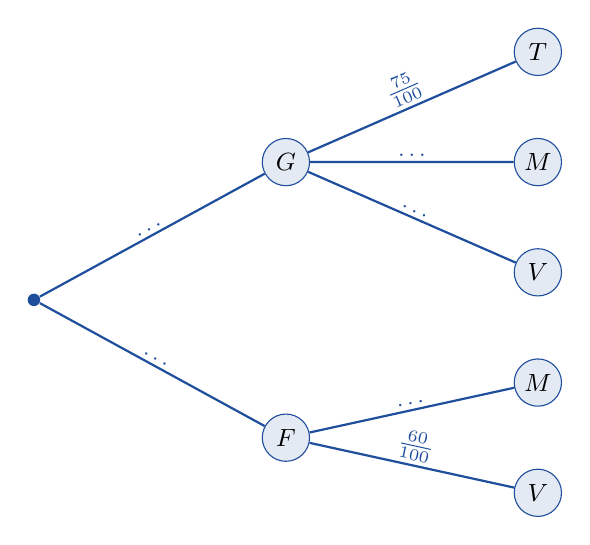
\begin{tikzpicture}[ev/.style={rounded rectangle,fill=cDef!12,draw=cDef,inner sep=2pt,minimum height=6mm,minimum width=7mm,font=\small},pb/.style={midway,above,sloped,font=\footnotesize,inner sep=1.5pt}]
\node[circle,fill=cDef,inner sep=1.6pt] (r) at (0,-3.15){};
\node[ev] (a0) at (3.20,-1.40){$G$};
\draw[cDef,thick] (r)--(a0) node[pb]{$\ldots$};
\node[ev] (b00) at (6.40,-0.00){$T$};
\draw[cDef,thick] (a0)--(b00) node[pb]{$\frac{75}{100}$};
\node[ev] (b01) at (6.40,-1.40){$M$};
\draw[cDef,thick] (a0)--(b01) node[pb]{$\ldots$};
\node[ev] (b02) at (6.40,-2.80){$V$};
\draw[cDef,thick] (a0)--(b02) node[pb]{$\ldots$};
\node[ev] (a1) at (3.20,-4.90){$F$};
\draw[cDef,thick] (r)--(a1) node[pb]{$\ldots$};
\node[ev] (b10) at (6.40,-4.20){$M$};
\draw[cDef,thick] (a1)--(b10) node[pb]{$\ldots$};
\node[ev] (b11) at (6.40,-5.60){$V$};
\draw[cDef,thick] (a1)--(b11) node[pb]{$\frac{60}{100}$};
\end{tikzpicture}\end{LTR}\end{center}
\end{tamrin}
\begin{hal}
\QQ{1} $P(G)=\dfrac{20}{35}=\dfrac47$ ، $P(F)=\dfrac{15}{35}=\dfrac37$ ، $P_F(M)=1-0{,}6=0{,}4$:
\par\begin{center}\begin{LTR}\begin{tikzpicture}[ev/.style={rounded rectangle,fill=cDef!12,draw=cDef,inner sep=2pt,minimum height=6mm,minimum width=7mm,font=\small},pb/.style={midway,above,sloped,font=\footnotesize,inner sep=1.5pt}]
\node[circle,fill=cDef,inner sep=1.6pt] (r) at (0,-3.15){};
\node[font=\small\bfseries,text=cSec] at (8.70,0.90){\ar{الاحتمال}};
\node[ev] (a0) at (3.20,-1.40){$G$};
\draw[cDef,thick] (r)--(a0) node[pb]{$\frac{20}{35}$};
\node[ev] (b00) at (6.40,-0.00){$T$};
\draw[cDef,thick] (a0)--(b00) node[pb]{$\frac{75}{100}$};
\node[font=\small] at (8.70,-0.00){$\frac37$};
\node[ev] (b01) at (6.40,-1.40){$M$};
\draw[cDef,thick] (a0)--(b01) node[pb]{$\frac{15}{100}$};
\node[font=\small] at (8.70,-1.40){$\frac{3}{35}$};
\node[ev] (b02) at (6.40,-2.80){$V$};
\draw[cDef,thick] (a0)--(b02) node[pb]{$\frac{10}{100}$};
\node[font=\small] at (8.70,-2.80){$\frac{2}{35}$};
\node[ev] (a1) at (3.20,-4.90){$F$};
\draw[cDef,thick] (r)--(a1) node[pb]{$\frac{15}{35}$};
\node[ev] (b10) at (6.40,-4.20){$M$};
\draw[cDef,thick] (a1)--(b10) node[pb]{$\frac{40}{100}$};
\node[font=\small] at (8.70,-4.20){$\frac{6}{35}$};
\node[ev] (b11) at (6.40,-5.60){$V$};
\draw[cDef,thick] (a1)--(b11) node[pb]{$\frac{60}{100}$};
\node[font=\small] at (8.70,-5.60){$\frac{9}{35}$};
\end{tikzpicture}\end{LTR}\end{center}
\QQ{2} $P(V)=\dfrac2{35}+\dfrac9{35}=\bx{\frac{11}{35}}$
\QQ{3} $P_V(G)=\dfrac{\frac2{35}}{\frac{11}{35}}=\bx{\frac2{11}}$
\QQ{4} $P(T)=P(G\cap T)=\dfrac37$ ، ومنه $P\big(\overline T\big)=1-\dfrac37=\bx{\frac47}$
\end{hal}
% ===================== 17 =====================
\begin{tamrin}{تمرين من بكالوريا 2012 -- الموضوع الثاني}
بيّنت دراسة إحصائية لتلاميذ السنة الثالثة ثانوي بإحدى الثانويات أن $30\%$ من التلاميذ قدموا من الإكمالية $A$ و $45\%$ من الإكمالية $B$ والبقية من الإكمالية $C$. بعد اجتياز التلاميذ للبكالوريا تبيّن ما يلي: نجح في الامتحان $25\%$ من التلاميذ القادمين من الإكمالية $A$ و $18\%$ من الذين قدموا من الإكمالية $B$ و $84\%$ من الذين قدموا من الإكمالية $C$.
\par نختار تلميذًا من تلاميذ السنة الثالثة ثانوي بطريقة عشوائية بعد اجتياز امتحان البكالوريا. نرمز بـ $R$ إلى الحادثة «التلميذ المختار نجح في الامتحان» ، وبـ $A$ ، $B$ ، $C$ إلى الحوادث «التلميذ المختار قادم من الإكمالية $A$» ، «$\ldots$ من الإكمالية $B$» ، «$\ldots$ من الإكمالية $C$».
\QQ{1} أنجز شجرة الاحتمالات التي تنمذج هذه الوضعية.
\QQ{2} أثبت أن $P(C\cap R)=0{,}21$.
\QQ{3} احسب $P(R)$ احتمال الحادثة $R$.
\QQ{4} احسب الاحتمال الشرطي $P_R(B)$.
\end{tamrin}
\begin{hal}
\QQ{1} $P(C)=1-0{,}3-0{,}45=0{,}25$:
\par\begin{center}\begin{LTR}\begin{tikzpicture}[ev/.style={rounded rectangle,fill=cDef!12,draw=cDef,inner sep=2pt,minimum height=6mm,minimum width=7mm,font=\small},pb/.style={midway,above,sloped,font=\footnotesize,inner sep=1.5pt}]
\node[circle,fill=cDef,inner sep=1.6pt] (r) at (0,-3.50){};
\node[font=\small\bfseries,text=cSec] at (8.70,0.90){\ar{الاحتمال}};
\node[ev] (a0) at (3.20,-0.70){$A$};
\draw[cDef,thick] (r)--(a0) node[pb]{$0,3$};
\node[ev] (b00) at (6.40,-0.00){$R$};
\draw[cDef,thick] (a0)--(b00) node[pb]{$0,25$};
\node[font=\small] at (8.70,-0.00){$0,075$};
\node[ev] (b01) at (6.40,-1.40){$\overline R$};
\draw[cDef,thick] (a0)--(b01) node[pb]{$0,75$};
\node[font=\small] at (8.70,-1.40){$0,225$};
\node[ev] (a1) at (3.20,-3.50){$B$};
\draw[cDef,thick] (r)--(a1) node[pb]{$0,45$};
\node[ev] (b10) at (6.40,-2.80){$R$};
\draw[cDef,thick] (a1)--(b10) node[pb]{$0,18$};
\node[font=\small] at (8.70,-2.80){$0,081$};
\node[ev] (b11) at (6.40,-4.20){$\overline R$};
\draw[cDef,thick] (a1)--(b11) node[pb]{$0,82$};
\node[font=\small] at (8.70,-4.20){$0,369$};
\node[ev] (a2) at (3.20,-6.30){$C$};
\draw[cDef,thick] (r)--(a2) node[pb]{$0,25$};
\node[ev] (b20) at (6.40,-5.60){$R$};
\draw[cDef,thick] (a2)--(b20) node[pb]{$0,84$};
\node[font=\small] at (8.70,-5.60){$0,21$};
\node[ev] (b21) at (6.40,-7.00){$\overline R$};
\draw[cDef,thick] (a2)--(b21) node[pb]{$0,16$};
\node[font=\small] at (8.70,-7.00){$0,04$};
\end{tikzpicture}\end{LTR}\end{center}
\QQ{2} $P(C\cap R)=0{,}25\times0{,}84=\bx{0{,}21}$
\QQ{3} $P(R)=0{,}075+0{,}081+0{,}21=\bx{0{,}366}$
\QQ{4} $P_R(B)=\dfrac{0{,}081}{0{,}366}=\bx{\frac{27}{122}}\approx0{,}22$
\end{hal}
% ===================== 18 =====================
\begin{tamrin}{تمرين من بكالوريا 2011 -- الموضوع الأول}
يتكون مجتمع من $55\%$ نساء و $45\%$ رجال. $25\%$ من النساء يتحدثن لغة أجنبية و $35\%$ من الرجال يتحدثون أيضًا لغة أجنبية. نختار عشوائيًا شخصًا من هذا المجتمع ونعتبر الحوادث التالية: $H$: «رجل» ، $F$: «امرأة» ، $A$: «رجل يتحدث لغة أجنبية» ، $B$: «امرأة تتحدث لغة أجنبية».
\QQ{1} أنقل شجرة الاحتمالات ثم أكملها.
\QQ{2} احسب احتمال أن يكون الشخص المختار:
\begin{sq}
\qa رجلًا يتحدث لغة أجنبية.
\qb امرأة لا تتحدث لغة أجنبية.
\qc شخصًا يتحدث لغة أجنبية.
\end{sq}
\QQ{3} احسب احتمال أن يكون الشخص المختار امرأة ، علمًا أنه يتحدث لغة أجنبية.
\par\begin{center}\begin{LTR}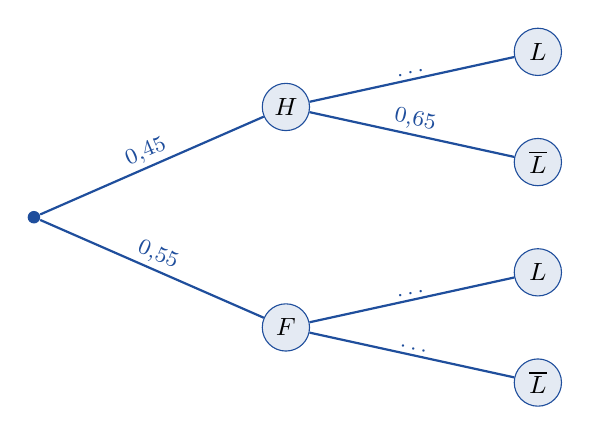
\begin{tikzpicture}[ev/.style={rounded rectangle,fill=cDef!12,draw=cDef,inner sep=2pt,minimum height=6mm,minimum width=7mm,font=\small},pb/.style={midway,above,sloped,font=\footnotesize,inner sep=1.5pt}]
\node[circle,fill=cDef,inner sep=1.6pt] (r) at (0,-2.10){};
\node[ev] (a0) at (3.20,-0.70){$H$};
\draw[cDef,thick] (r)--(a0) node[pb]{$0,45$};
\node[ev] (b00) at (6.40,-0.00){$L$};
\draw[cDef,thick] (a0)--(b00) node[pb]{$\ldots$};
\node[ev] (b01) at (6.40,-1.40){$\overline L$};
\draw[cDef,thick] (a0)--(b01) node[pb]{$0,65$};
\node[ev] (a1) at (3.20,-3.50){$F$};
\draw[cDef,thick] (r)--(a1) node[pb]{$0,55$};
\node[ev] (b10) at (6.40,-2.80){$L$};
\draw[cDef,thick] (a1)--(b10) node[pb]{$\ldots$};
\node[ev] (b11) at (6.40,-4.20){$\overline L$};
\draw[cDef,thick] (a1)--(b11) node[pb]{$\ldots$};
\end{tikzpicture}\end{LTR}\end{center}
\end{tamrin}
\begin{hal}
\QQ{1} نرمز بـ $L$ للحادثة «الشخص يتحدث لغة أجنبية» ، فيكون $A=H\cap L$ و $B=F\cap L$:
\par\begin{center}\begin{LTR}\begin{tikzpicture}[ev/.style={rounded rectangle,fill=cDef!12,draw=cDef,inner sep=2pt,minimum height=6mm,minimum width=7mm,font=\small},pb/.style={midway,above,sloped,font=\footnotesize,inner sep=1.5pt}]
\node[circle,fill=cDef,inner sep=1.6pt] (r) at (0,-2.10){};
\node[font=\small\bfseries,text=cSec] at (8.70,0.90){\ar{الاحتمال}};
\node[ev] (a0) at (3.20,-0.70){$H$};
\draw[cDef,thick] (r)--(a0) node[pb]{$0,45$};
\node[ev] (b00) at (6.40,-0.00){$L$};
\draw[cDef,thick] (a0)--(b00) node[pb]{$0,35$};
\node[font=\small] at (8.70,-0.00){$0,1575$};
\node[ev] (b01) at (6.40,-1.40){$\overline L$};
\draw[cDef,thick] (a0)--(b01) node[pb]{$0,65$};
\node[font=\small] at (8.70,-1.40){$0,2925$};
\node[ev] (a1) at (3.20,-3.50){$F$};
\draw[cDef,thick] (r)--(a1) node[pb]{$0,55$};
\node[ev] (b10) at (6.40,-2.80){$L$};
\draw[cDef,thick] (a1)--(b10) node[pb]{$0,25$};
\node[font=\small] at (8.70,-2.80){$0,1375$};
\node[ev] (b11) at (6.40,-4.20){$\overline L$};
\draw[cDef,thick] (a1)--(b11) node[pb]{$0,75$};
\node[font=\small] at (8.70,-4.20){$0,4125$};
\end{tikzpicture}\end{LTR}\end{center}
\QQ{2}
\pa $P(A)=P(H\cap L)=0{,}45\times0{,}35=\bx{0{,}1575}$
\pb $P\big(F\cap\overline L\big)=0{,}55\times0{,}75=\bx{0{,}4125}$
\pc $P(L)=0{,}1575+0{,}1375=\bx{0{,}295}$
\QQ{3} $P_L(F)=\dfrac{0{,}1375}{0{,}295}=\bx{\frac{55}{118}}\approx0{,}47$
\end{hal}
% ===================== 19 =====================
\begin{tamrin}{تمرين من بكالوريا 2011 -- الموضوع الثاني}
عدد تلاميذ ثانوية هو $900$ ، يتوزعون حسب المستوى والصنف (داخلي أو خارجي) كما يلي:
\begin{center}\begin{LTR}\renewcommand{\arraystretch}{1.4}
\begin{tabular}{|C|c|c|c|c|}\hline
\rowcolor{cSec!12}الصنف & \ar{السنة الأولى} & \ar{السنة الثانية} & \ar{السنة الثالثة} & \ar{المجموع}\\\hline
خارجيون & $250$ & $200$ & $150$ & $600$\\\hline
داخليون & $100$ & $120$ & $80$ & $300$\\\hline
المجموع & $350$ & $320$ & $230$ & $900$\\\hline
\end{tabular}\end{LTR}\end{center}
نختار تلميذًا بطريقة عشوائية. احسب الاحتمالات التالية:
\QQ{1} احتمال أن يكون التلميذ خارجيًا.
\QQ{2} احتمال أن يكون التلميذ من السنة الأولى.
\QQ{3} احتمال أن يكون التلميذ من السنة الأولى وخارجيًا.
\QQ{4} احتمال أن يكون التلميذ من السنة الأولى علمًا أنه خارجي.
\QQ{5} هل الحادثتان «التلميذ من السنة الأولى» و «التلميذ خارجي» مستقلتان؟
\end{tamrin}
\begin{hal}
نرمز بـ $E$ للخارجي و $P_1$ لتلميذ السنة الأولى.
\QQ{1} $P(E)=\dfrac{600}{900}=\bx{\frac23}$ \qquad \QQ{2} $P(P_1)=\dfrac{350}{900}=\bx{\frac7{18}}$ \qquad \QQ{3} $P(P_1\cap E)=\dfrac{250}{900}=\bx{\frac5{18}}$
\QQ{4} $P_E(P_1)=\dfrac{250}{600}=\bx{\frac5{12}}$
\QQ{5} $P(P_1)\times P(E)=\dfrac7{18}\times\dfrac23=\dfrac7{27}\neq\dfrac5{18}=P(P_1\cap E)$: \bxt{الحادثتان غير مستقلتين}.
\end{hal}
% ===================== 20 =====================
\begin{tamrin}{تمرين من بكالوريا 2009 -- الموضوع الأول}
يحتوي كيس على $9$ كرات متماثلة لا نفرق بينها باللمس ، منها $4$ كرات بيضاء تحمل الأرقام $1$ ، $2$ ، $3$ ، $3$ و $5$ كرات حمراء تحمل الأرقام $1$ ، $1$ ، $2$ ، $2$ ، $3$. نسحب عشوائيًا من هذا الكيس كرتين على التوالي مع إرجاع الكرة المسحوبة.
\QQ{1} شكّل شجرة الاحتمالات الموافقة لهذه الوضعية في الحالتين الآتيتين: باعتماد ألوان الكرات ؛ باعتماد الأرقام المسجلة على الكرات.
\QQ{2} احسب احتمال كل من الحوادث التالية: $A$: «الكرتان المسحوبتان بيضاوان» ؛ $B$: «إحدى الكرتين المسحوبتين فقط حمراء» ؛ $C$: «لا يظهر الرقم $1$».
\end{tamrin}
\begin{hal}
\QQ{1} \textbf{باعتماد الألوان} ($W$: بيضاء ، $R$: حمراء) ، مع الإرجاع فالسحبان متماثلان:
\par\begin{center}\begin{LTR}\begin{tikzpicture}[ev/.style={rounded rectangle,fill=cDef!12,draw=cDef,inner sep=2pt,minimum height=6mm,minimum width=7mm,font=\small},pb/.style={midway,above,sloped,font=\footnotesize,inner sep=1.5pt}]
\node[circle,fill=cDef,inner sep=1.6pt] (r) at (0,-2.10){};
\node[font=\small\bfseries,text=cSec] at (8.70,0.90){\ar{الاحتمال}};
\node[ev] (a0) at (3.20,-0.70){$W$};
\draw[cDef,thick] (r)--(a0) node[pb]{$\frac49$};
\node[ev] (b00) at (6.40,-0.00){$W$};
\draw[cDef,thick] (a0)--(b00) node[pb]{$\frac49$};
\node[font=\small] at (8.70,-0.00){$\frac{16}{81}$};
\node[ev] (b01) at (6.40,-1.40){$R$};
\draw[cDef,thick] (a0)--(b01) node[pb]{$\frac59$};
\node[font=\small] at (8.70,-1.40){$\frac{20}{81}$};
\node[ev] (a1) at (3.20,-3.50){$R$};
\draw[cDef,thick] (r)--(a1) node[pb]{$\frac59$};
\node[ev] (b10) at (6.40,-2.80){$W$};
\draw[cDef,thick] (a1)--(b10) node[pb]{$\frac49$};
\node[font=\small] at (8.70,-2.80){$\frac{20}{81}$};
\node[ev] (b11) at (6.40,-4.20){$R$};
\draw[cDef,thick] (a1)--(b11) node[pb]{$\frac59$};
\node[font=\small] at (8.70,-4.20){$\frac{25}{81}$};
\end{tikzpicture}\end{LTR}\end{center}
\textbf{باعتماد الأرقام:} الرقم $1$ على $3$ كرات ، الرقم $2$ على $3$ كرات ، الرقم $3$ على $3$ كرات ، فكل رقم احتماله $\dfrac39=\dfrac13$:
\par\begin{center}\begin{LTR}\begin{tikzpicture}[ev/.style={rounded rectangle,fill=cDef!12,draw=cDef,inner sep=2pt,minimum height=6mm,minimum width=7mm,font=\small},pb/.style={midway,above,sloped,font=\footnotesize,inner sep=1.5pt}]
\node[circle,fill=cDef,inner sep=1.6pt] (r) at (0,-5.60){};
\node[font=\small\bfseries,text=cSec] at (8.70,0.90){\ar{الاحتمال}};
\node[ev] (a0) at (3.20,-1.40){$1$};
\draw[cDef,thick] (r)--(a0) node[pb]{$\frac13$};
\node[ev] (b00) at (6.40,-0.00){$1$};
\draw[cDef,thick] (a0)--(b00) node[pb]{$\frac13$};
\node[font=\small] at (8.70,-0.00){$\frac19$};
\node[ev] (b01) at (6.40,-1.40){$2$};
\draw[cDef,thick] (a0)--(b01) node[pb]{$\frac13$};
\node[font=\small] at (8.70,-1.40){$\frac19$};
\node[ev] (b02) at (6.40,-2.80){$3$};
\draw[cDef,thick] (a0)--(b02) node[pb]{$\frac13$};
\node[font=\small] at (8.70,-2.80){$\frac19$};
\node[ev] (a1) at (3.20,-5.60){$2$};
\draw[cDef,thick] (r)--(a1) node[pb]{$\frac13$};
\node[ev] (b10) at (6.40,-4.20){$1$};
\draw[cDef,thick] (a1)--(b10) node[pb]{$\frac13$};
\node[font=\small] at (8.70,-4.20){$\frac19$};
\node[ev] (b11) at (6.40,-5.60){$2$};
\draw[cDef,thick] (a1)--(b11) node[pb]{$\frac13$};
\node[font=\small] at (8.70,-5.60){$\frac19$};
\node[ev] (b12) at (6.40,-7.00){$3$};
\draw[cDef,thick] (a1)--(b12) node[pb]{$\frac13$};
\node[font=\small] at (8.70,-7.00){$\frac19$};
\node[ev] (a2) at (3.20,-9.80){$3$};
\draw[cDef,thick] (r)--(a2) node[pb]{$\frac13$};
\node[ev] (b20) at (6.40,-8.40){$1$};
\draw[cDef,thick] (a2)--(b20) node[pb]{$\frac13$};
\node[font=\small] at (8.70,-8.40){$\frac19$};
\node[ev] (b21) at (6.40,-9.80){$2$};
\draw[cDef,thick] (a2)--(b21) node[pb]{$\frac13$};
\node[font=\small] at (8.70,-9.80){$\frac19$};
\node[ev] (b22) at (6.40,-11.20){$3$};
\draw[cDef,thick] (a2)--(b22) node[pb]{$\frac13$};
\node[font=\small] at (8.70,-11.20){$\frac19$};
\end{tikzpicture}\end{LTR}\end{center}
\QQ{2} $P(A)=\dfrac49\times\dfrac49=\bx{\frac{16}{81}}$ \ ؛ \ $P(B)=\dfrac{20}{81}+\dfrac{20}{81}=\bx{\frac{40}{81}}$ \ ؛ \ $P(C)=\dfrac23\times\dfrac23=\bx{\frac49}$
\end{hal}
% ===================== 21 =====================
\begin{tamrin}{تمرين من بكالوريا 2008 -- الموضوع الأول}
يحتوي كيس على $7$ كرات منها $3$ بيضاء تحمل الأرقام $-2$ ، $1$ ، $2$ وأربع حمراء تحمل الأرقام $1$ ، $1$ ، $2$ ، $2$.
\QQ{1} نسحب كرة واحدة من الكيس.
\begin{sq}
\qa ما احتمال الحصول على كرة تحمل الرقم $1$ ؟
\qb إذا كانت الكرة المسحوبة تحمل الرقم $1$ فما هو احتمال أن يكون لونها أحمر؟
\end{sq}
\QQ{2} نسحب على التوالي كرتين من الكيس دون إرجاع.
\begin{sq}
\qa ما احتمال الحصول على كرتين تحمل كل منهما رقمًا فرديًا؟
\qb ما احتمال الحصول على كرتين من نفس اللون؟
\qc ما احتمال أن يكون مجموع الرقمين الظاهرين $3$ ؟
\end{sq}
\end{tamrin}
\begin{hal}
\QQ{1}
\pa الرقم $1$ على $3$ كرات (بيضاء وحمراوان): \ $P=\bx{\frac37}$
\pb من بين الكرات الثلاث التي تحمل $1$ ، اثنتان حمراوان: \ $P=\bx{\frac23}$
\QQ{2} سحب على التوالي دون إرجاع: $\text{card}\,\Omega=7\times6=42$.
\pa الكرات ذات الرقم الفردي: $3$ (التي تحمل $1$): \ $P=\dfrac{3\times2}{42}=\bx{\frac17}$
\pb بيضاوان: $3\times2=6$ ، حمراوان: $4\times3=12$: \ $P=\dfrac{18}{42}=\bx{\frac37}$
\pc المجموع $3$: رقم $1$ ورقم $2$ (بأي ترتيب) ، والرقم $2$ على $3$ كرات: $3\times3\times2=18$: \ $P=\dfrac{18}{42}=\bx{\frac37}$
\end{hal}
% ===================== 22 =====================
\begin{tamrin}{تمرين من بكالوريا 2008 -- الموضوع الثاني}
يحتوي كيس على $10$ قريصات لا يمكن التفريق بينها باللمس ، من بينها $6$ حمراء اللون تحمل الأرقام $1$ ، $2$ ، $2$ ، $4$ ، $6$ ، $8$ والبقية بيضاء تحمل الأرقام $1$ ، $3$ ، $5$ ، $5$. نسحب ثلاث قريصات من هذا الكيس واحدة تلو الأخرى دون إرجاع. المطلوب حساب:
\begin{sq}
\qa احتمال الحصول على ثلاث قريصات من نفس اللون.
\qb احتمال الحصول على ثلاث قريصات بلونين مختلفين.
\qc احتمال الحصول على ثلاث قريصات تحمل ثلاثة أرقام مجموعها $15$.
\qd احتمال الحصول على ثلاث قريصات مجموعها $15$ علمًا أنها من نفس اللون.
\end{sq}
\end{tamrin}
\begin{hal}
السحب على التوالي دون إرجاع: $\text{card}\,\Omega=10\times9\times8=720$.
\pa حمراء: $6\times5\times4=120$ ، بيضاء: $4\times3\times2=24$: \ $P=\dfrac{144}{720}=\bx{\frac15}$
\pb الحادثة العكسية: $P=1-\dfrac15=\bx{\frac45}$
\pc الثلاثيات (دون ترتيب) التي مجموعها $15$:
\begin{center}\begin{LTR}\renewcommand{\arraystretch}{1.4}
\begin{tabular}{|C|c|c|c|c|c|c|}\hline
\rowcolor{cSec!12}الأرقام & $1+6+8$ & $2+8+5$ & $4+6+5$ & $4+8+3$ & $6+8+1$ & \ar{المجموع}\\\hline
الألوان & \ar{ح ح ح} & \ar{ح ح ب} & \ar{ح ح ب} & \ar{ح ح ب} & \ar{ح ح ب} & \\\hline
عدد الاختيارات & $1$ & $2\times2=4$ & $2$ & $1$ & $1$ & $9$\\\hline
\end{tabular}\end{LTR}\end{center}
كل اختيار يعطي $3!=6$ ترتيبات: $9\times6=54$: \quad $P=\dfrac{54}{720}=\bx{\frac3{40}}$
\pd من نفس اللون ومجموعها $15$: الثلاثية الحمراء $\{1;6;8\}$ فقط ، أي $6$ ترتيبات:
\[P=\frac{\frac{6}{720}}{\frac{144}{720}}=\frac6{144}=\bx{\frac1{24}}\]
\end{hal}
\end{document}
